\documentclass[11pt]{article}
\makeatletter\def\input@path{{../}}\makeatother
\usepackage{preamble}
\renewcommand{\chaptername}{Chapter 2: From prior information to posterior inference}
\graphicspath{{figures/}}

\begin{document}

% ================================================================= title page
\begin{titlepage}
\centering
\vspace*{3cm}
{\color{book}\large Worked solutions to}\\[0.6em]
{\Huge\bfseries\color{navy} Bayesian Statistical Methods}\\[0.4em]
{\large\color{book} With Applications to Machine Learning --- Reich \& Ghosh (2nd ed.)}\\[2.5cm]
{\color{navy}\rule{0.6\linewidth}{1pt}}\\[1em]
{\huge Chapter 2}\\[0.4em]
{\LARGE\itshape From prior information to posterior inference}\\[1em]
{\color{navy}\rule{0.6\linewidth}{1pt}}\\[2.5cm]
\begin{minipage}{0.78\linewidth}
\small
Every exercise is presented in the same order:
\begin{enumerate}[leftmargin=1.5em]
  \item[\color{book}\faBook] the \textbf{exact} exercise text from the book;
  \item[\color{mine}\faComment*] the problem \textbf{in plain words};
  \item[\color{idea}\faLightbulb] the \textbf{key idea} you need;
  \item[\color{navy}\faPencil*] a step-by-step \textbf{solution};
  \item[\color{ans}\faCheckCircle] the boxed \textbf{answer};
  \item[\color{warn}\faExclamationTriangle] \textbf{takeaways} and common mistakes.
\end{enumerate}
All numbers and figures are reproduced by \texttt{ch02/code/ch02.R}.
\end{minipage}
\vfill
{\small\color{book} Sai Sridhar \quad$\cdot$\quad \today}
\end{titlepage}

\tableofcontents
\clearpage

\section*{Answers at a glance}
\addcontentsline{toc}{section}{Answers at a glance}
\begin{center}
\small
\renewcommand{\arraystretch}{1.25}
\begin{tabular}{>{\bfseries\color{navy}}r p{0.82\linewidth}}\toprule
1  & $\frac{n\bar Y}{n+m}\pm1.96\frac{\sigma}{\sqrt{n+m}}$; $m=0$ gives exact 95\% coverage for every $\mu$.\\
2  & Regular $\approx0.200$, World Series $\approx0.371$ HR/game; $\Prob(\lambda_{WS}>\lambda_{R})\approx0.95$ --- suggestive, not conclusive.\\
3  & $\theta\sim\dist{Gamma}(a,b)\Rightarrow\theta\mid Y\sim\dist{Gamma}(a+1,\,b+Y)$.\\
4  & $\lambda\mid\mathbf Y\sim\dist{Gamma}(30.1,6.1)$; $\Prob(\lambda>4\mid\mathbf Y)\approx0.85$.\\
5  & $\dist{Beta}(a+m,\,b+Y)=\dist{Beta}(6,11)$; 95\% CI $(0.152,0.587)$.\\
6  & $\E(\theta\mid y)=12.8+0.8y$; spurious ``effect'' $\approx6.0$ bpm; fix with a randomised control group.\\
7  & $\dist{Gamma}(56.9,\ 0.754)$: SD 10, median 75.\\
8  & $\Prob(\sigma>1)\approx0.225$ vs $0.237$ (ratio 0.95); $\Prob(\sigma>2)\approx2.6\times10^{-5}$ vs $1.4\times10^{-5}$ (ratio 1.77).\\
9  & $c\approx1.3$; that is \emph{not} uninformative for $\alpha,\beta$.\\
10 & $\dist{Gamma}(44.01,50.01)$: mean 0.88, CI $(0.64,1.16)$; Poisson fits badly; $\Prob(\lambda>1)\approx0.18$.\\
11 & Geometric; prior $\Prob(Y\ge7)=1/8$; posterior $\dist{Beta}(2,6)$; PPD $=3/13\approx0.231$.\\
12 & $\lambda\mid\text{data}\sim\dist{Gamma}(a+7,\ b+95.9)$; mean $\approx0.073$/week.\\
13 & Experts: $\dist{Beta}(17.1,0.9)$, $\dist{Beta}(2.4,0.6)$; posterior mixture weights $0.62/0.38$.\\
14 & No prior is flat on both $\theta$ and the odds $\gamma$.\\
15 & $p(\mu\mid Y)\propto e^{-(Y-\mu)^2/2}$ integrates to $\sqrt{2\pi}$: $\mu\mid Y\sim\dist{N}(Y,1)$.\\
16 & $m(Y)\ge c(Y)\int\pi(\theta)\dd\theta=\infty$.\\
17 & $f(\mathbf y\mid\theta)\ge\prod_i 0.5\phi(y_i)>0$, then apply Exercise 16.\\
18 & $\Prob(\delta>0\mid z=2)=0.955$ (mixture) vs $0.977$ (vague prior).\\
19 & $\pi(\lambda)\propto\lambda^{-1/2}$, improper; posterior $\dist{Gamma}(Y+\frac12,1)$, proper for every $Y\ge0$.\\
20 & $\pi(\lambda)\propto\lambda^{-1}$, improper; posterior $\dist{Gamma}(1,Y)$, proper iff $Y>0$.\\
21 & Jeffreys: $\lambda\mid Y\sim\dist{Gamma}(10.5,1)$, mean 10.5, CI $(5.1,17.7)$.\\
22 & EB prior $\dist{Beta}(5.43,5.89)$ shrinks small counties toward 0.48 and narrows the intervals.\\\bottomrule
\end{tabular}
\end{center}
\clearpage

% ================================================================= Exercise 1
\exercise{2.1 --- Frequentist coverage of a Bayesian interval}

\begin{problem}{1}
Assume $Y_1,\dots,Y_n|\mu\iid\dist{Normal}(\mu,\sigma^2)$ where $\sigma^2$ is fixed and the unknown mean $\mu$ has prior $\mu\sim\dist{Normal}(0,\sigma^2/m)$.
\begin{enumerate}[(a)]
\item Give a 95\% posterior interval for $\mu$.
\item Select a value of $m$, and argue that for this choice your 95\% posterior credible interval has frequentist coverage 0.95. That is, if you draw many samples of size $n$ and compute the 95\% interval following the formula in (a) for each sample, in the long-run 95\% of the intervals will contain the true value of $\mu$.
\end{enumerate}
\end{problem}

\begin{restate}
Work out the posterior of a normal mean under a normal prior, write down its 95\% credible interval, then find the prior strength $m$ for which this Bayesian interval also behaves like a classical 95\% confidence interval.
\end{restate}

\begin{keyidea}
\textbf{Normal--normal conjugacy}: precisions (1/variance) add, and the posterior mean is a precision-weighted average. The prior $\dist{Normal}(0,\sigma^2/m)$ is worth $m$ ``pseudo-observations'' equal to 0.
\end{keyidea}

\solution
\step{(a) Posterior.}
Likelihood precision $n/\sigma^2$ (from $\bar Y\sim\dist N(\mu,\sigma^2/n)$), prior precision $m/\sigma^2$. Adding:
\[
\mu\mid\mathbf Y\sim\dist{Normal}\!\left(\frac{n\bar Y+m\cdot0}{n+m},\ \frac{\sigma^2}{n+m}\right).
\]
A 95\% (equal-tailed $=$ HPD, by symmetry) interval is
\[
\frac{n\bar Y}{n+m}\ \pm\ 1.96\,\frac{\sigma}{\sqrt{n+m}}.
\]

\step{(b) Choose $m=0$.}
Then the interval is $\bar Y\pm1.96\,\sigma/\sqrt n$. In repeated sampling with the true $\mu$ fixed, $\bar Y\sim\dist N(\mu,\sigma^2/n)$, so
\[
\Prob\Big(|\bar Y-\mu|\le1.96\tfrac{\sigma}{\sqrt n}\Big)=\Prob(|Z|\le1.96)=0.95\quad\text{for every }\mu.
\]
$m=0$ is the limit of an infinitely vague prior (the flat improper prior $\pi(\mu)\propto1$).

\step{Why other $m$ fail.} For general $m$, $\frac{n\bar Y}{n+m}-\mu\sim\dist N\big(-\frac{m\mu}{n+m},\frac{n\sigma^2}{(n+m)^2}\big)$, so the coverage is
\[
C(\mu)=\Phi\!\Big(1.96\sqrt{\tfrac{n+m}{n}}+\tfrac{m\mu}{\sqrt n\,\sigma}\Big)-\Phi\!\Big(-1.96\sqrt{\tfrac{n+m}{n}}+\tfrac{m\mu}{\sqrt n\,\sigma}\Big).
\]
This is above 0.95 near $\mu=0$ (the prior is right, and the interval is wider than needed) and collapses when $\mu$ is far from 0 (the interval is shrunk toward the wrong place). For $n=10$, $\sigma=1$:
\begin{center}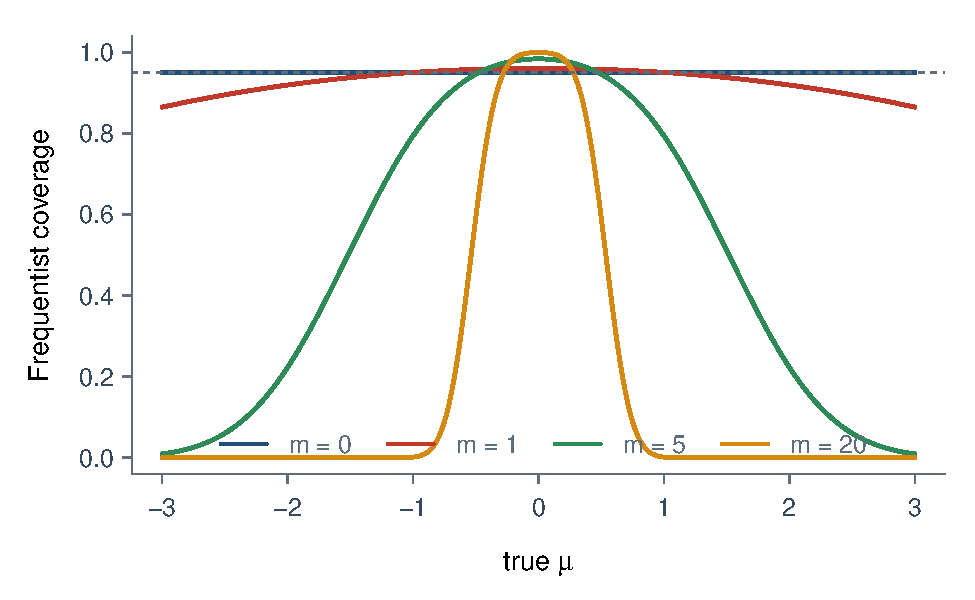
\includegraphics[width=0.72\linewidth]{ex01_coverage.pdf}\end{center}
A simulation with $m=0$, $\mu=1.7$ and $10^5$ samples gives coverage 0.9494.

\begin{answer}
(a) $\displaystyle \frac{n\bar Y}{n+m}\pm1.96\frac{\sigma}{\sqrt{n+m}}$. \qquad
(b) $m=0$: the interval becomes $\bar Y\pm1.96\sigma/\sqrt n$, whose coverage is exactly 0.95 for every $\mu$.
\end{answer}

\begin{takeaway}
A credible interval is a statement about $\mu$ \emph{given the data}; a confidence interval is a statement about the \emph{procedure}. They coincide for a flat prior here. With an informative prior, the average coverage over the prior is still 95\%, but not for every fixed $\mu$.
\end{takeaway}

% ================================================================= Exercise 2
\exercise{2.2 --- Is Reggie Jackson really ``Mr.\ October''?}

\begin{problem}{2}
The Major League Baseball player Reggie Jackson is known as ``Mr. October'' for his outstanding performances in the World Series (which takes place in October). Over his long career he played in 2820 regular-season games and hit 563 home runs in these games (a player can hit 0, 1, 2, \dots{} home runs in a game). He also played in 27 World Series games and hit 10 home runs in these games. Assuming uninformative conjugate priors, summarize the posterior distribution of his home-run rate in the regular season and World Series. Is there sufficient evidence to claim that he performs better in the World Series?
\end{problem}

\begin{restate}
Estimate his home runs per game in regular-season games and in World Series games, and judge whether the World Series rate is convincingly higher.
\end{restate}

\begin{keyidea}
Counts per game $\Rightarrow$ \textbf{Poisson--gamma}: if $Y_i\iid\dist{Poisson}(\lambda)$ for $n$ games and $\lambda\sim\dist{Gamma}(a,b)$, then $\lambda\mid\mathbf Y\sim\dist{Gamma}(a+\sum Y_i,\ b+n)$. Only the total and the number of games matter. To compare two rates, draw from both posteriors (Monte Carlo).
\end{keyidea}

\solution
\step{Prior.} $\dist{Gamma}(0.01,0.01)$ for each rate: mean 1 but variance 100, i.e.\ worth 0.01 games of data.
\step{Posteriors.}
\begin{center}
\begin{tabular}{lcccc}\toprule
 & Posterior & Mean & SD & 95\% interval\\\midrule
Regular season & $\dist{Gamma}(563.01,\ 2820.01)$ & 0.200 & 0.008 & (0.184, 0.217)\\
World Series & $\dist{Gamma}(10.01,\ 27.01)$ & 0.371 & 0.117 & (0.178, 0.633)\\\bottomrule
\end{tabular}
\end{center}
\begin{center}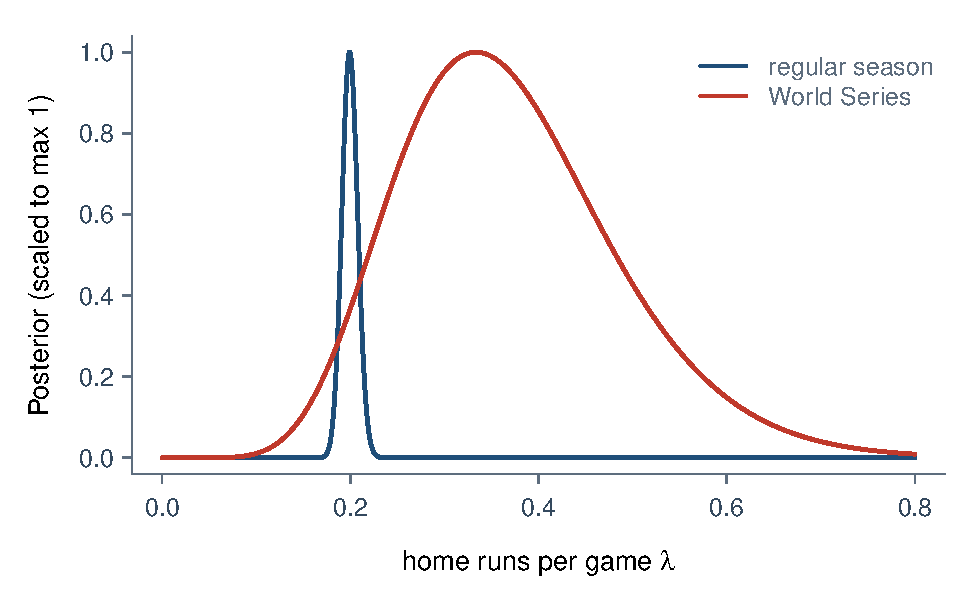
\includegraphics[width=0.7\linewidth]{ex02_reggie.pdf}\end{center}
\step{Comparison.} Drawing $10^6$ values from each posterior,
\[
\Prob(\lambda_{WS}>\lambda_{R}\mid\text{data})\approx0.951,\qquad
\frac{\lambda_{WS}}{\lambda_R}:\ \text{median }1.80,\ \text{95\% interval }(0.89,\ 3.19).
\]

\begin{answer}
Regular season $\approx0.200$ HR/game (0.184--0.217); World Series $\approx0.371$ HR/game (0.178--0.633). There is a 95\% posterior probability his World Series rate is higher, but the 95\% interval for the ratio still includes 1. The evidence is \textbf{suggestive but not conclusive}: 27 games is a small sample.
\end{answer}

\begin{takeaway}
Watch for \textbf{selection bias}: he got the nickname \emph{because} of a few spectacular games (three home runs in Game 6 of 1977). Testing a hypothesis on the same data that suggested it overstates the evidence.
\end{takeaway}

% ================================================================= Exercise 3
\exercise{2.3 --- Conjugate prior for the exponential rate}

\begin{problem}{3}
Assume that $Y|\theta\sim\dist{Exponential}(\theta)$, i.e., $Y|\theta\sim\dist{Gamma}(1,\theta)$. Find a conjugate prior distribution for $\theta$, and derive the resulting posterior distribution.
\end{problem}

\begin{restate}
Find a family of priors such that, after observing an exponential waiting time, the posterior stays in the same family.
\end{restate}

\begin{keyidea}
Write the likelihood \emph{as a function of $\theta$} and ask which density has the same shape. $\theta e^{-\theta y}$ looks like $\theta^{a-1}e^{-b\theta}$: a \textbf{Gamma kernel}.
\end{keyidea}

\solution
\step{Likelihood.} $f(Y\mid\theta)=\theta e^{-\theta Y}$, $Y>0$.
\step{Prior.} Try $\theta\sim\dist{Gamma}(a,b)$: $\pi(\theta)\propto\theta^{a-1}e^{-b\theta}$.
\step{Posterior.}
\[
p(\theta\mid Y)\propto\theta e^{-\theta Y}\cdot\theta^{a-1}e^{-b\theta}=\theta^{(a+1)-1}e^{-(b+Y)\theta}
\quad\Rightarrow\quad\theta\mid Y\sim\dist{Gamma}(a+1,\ b+Y).
\]
\step{With $n$ observations.} The same algebra gives $\theta\mid\mathbf Y\sim\dist{Gamma}\big(a+n,\ b+\sum_iY_i\big)$.

\begin{answer}
The Gamma family is conjugate: $\theta\sim\dist{Gamma}(a,b)\Rightarrow\theta\mid Y\sim\dist{Gamma}(a+1,\,b+Y)$; for $n$ observations, $\dist{Gamma}(a+n,\,b+\sum Y_i)$.
\end{answer}

\begin{takeaway}
Interpretation: $a$ acts as a prior number of events and $b$ as prior total waiting time. Posterior mean $\frac{a+n}{b+\sum Y_i}$ is ``events $\div$ time''.
\end{takeaway}

% ================================================================= Exercise 4
\exercise{2.4 --- Factory injury rate}

\begin{problem}{4}
A large factory's objective is to keep the injury rate below 4 injuries per month. In the past 6 months there have been 4, 5, 2, 7, 6 and 6 injuries. Conduct a Bayesian analysis of these data and compute the posterior probability that the injury rate exceeds four injuries per month.
\end{problem}

\begin{restate}
From six monthly injury counts, estimate the monthly rate and how likely it is to exceed the target of 4.
\end{restate}

\begin{keyidea}
Monthly counts $\Rightarrow$ Poisson likelihood; a vague Gamma prior gives a Gamma posterior. The answer is a tail probability $\Prob(\lambda>4\mid\mathbf Y)$.
\end{keyidea}

\solution
\step{Model.} $Y_t\mid\lambda\iid\dist{Poisson}(\lambda)$, $\lambda\sim\dist{Gamma}(0.1,0.1)$.
\step{Posterior.} $\sum Y_t=30$, $n=6$, so $\lambda\mid\mathbf Y\sim\dist{Gamma}(30.1,\ 6.1)$: mean 4.93, 95\% interval $(3.33,\ 6.85)$.
\begin{center}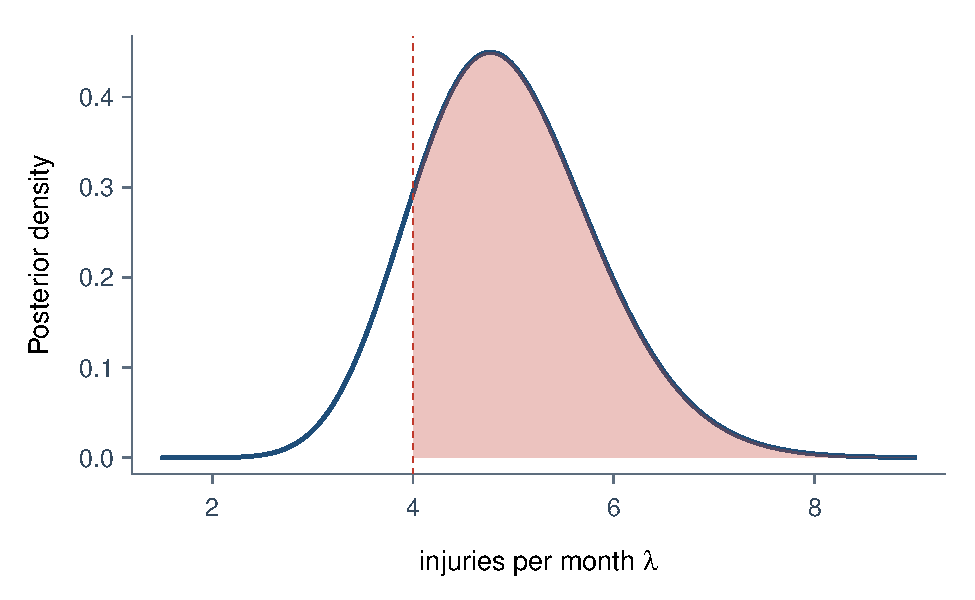
\includegraphics[width=0.68\linewidth]{ex04_injuries.pdf}\end{center}
\step{Tail probability.} $\Prob(\lambda>4\mid\mathbf Y)=$ \texttt{pgamma(4, 30.1, 6.1, lower.tail = FALSE)} $=0.853$.
\step{Sensitivity.}
\begin{center}
\begin{tabular}{lccc}\toprule
Prior & Posterior & Mean & $\Prob(\lambda>4\mid\mathbf Y)$\\\midrule
$\dist{Gamma}(0.01,0.01)$ & $\dist{Gamma}(30.01,6.01)$ & 4.99 & 0.867\\
$\dist{Gamma}(0.1,0.1)$ & $\dist{Gamma}(30.1,6.1)$ & 4.93 & 0.853\\
$\dist{Gamma}(1,1)$ & $\dist{Gamma}(31,7)$ & 4.43 & 0.690\\\bottomrule
\end{tabular}
\end{center}

\begin{answer}
$\lambda\mid\mathbf Y\sim\dist{Gamma}(30.1,6.1)$, posterior mean $\approx4.9$ injuries/month, and $\Prob(\lambda>4\mid\mathbf Y)\approx\mathbf{0.85}$. The factory is probably missing its target.
\end{answer}

\begin{takeaway}
With only six months of data the prior matters: $\dist{Gamma}(1,1)$ acts like an extra month with one injury and pulls the probability down to 0.69. Always report which prior you used.
\end{takeaway}

% ================================================================= Exercise 5
\exercise{2.5 --- Negative binomial likelihood with a beta prior}

\begin{problem}{5}
Assume that $Y|\theta\sim\dist{NegBinomial}(\theta,m)$ (see Appendix A.1) and $\theta\sim\dist{Beta}(a,b)$.
\begin{enumerate}[(a)]
\item Derive the posterior of $\theta$.
\item Plot the posterior of $\theta$, and give its 95\% credible interval assuming $m=5$, $Y=10$, and $a=b=1$.
\end{enumerate}
\end{problem}

\begin{restate}
$Y$ counts the failures before the $m$-th success. With a beta prior on the success probability, find the posterior and evaluate it for $m=5$, $Y=10$.
\end{restate}

\begin{keyidea}
Appendix A.1: $\Prob(Y=y\mid\theta)=\binom{y+m-1}{y}\theta^m(1-\theta)^y$. As a function of $\theta$ this is a Beta kernel, so the Beta prior is conjugate.
\end{keyidea}

\solution
\step{(a)}
\[
p(\theta\mid Y)\propto\theta^m(1-\theta)^Y\cdot\theta^{a-1}(1-\theta)^{b-1}=\theta^{a+m-1}(1-\theta)^{b+Y-1}
\ \Rightarrow\ \theta\mid Y\sim\dist{Beta}(a+m,\ b+Y).
\]
\step{(b)} $\dist{Beta}(1+5,\ 1+10)=\dist{Beta}(6,11)$: mean $6/17=0.353$, 95\% interval $(0.152,\ 0.587)$ (shaded).
\begin{center}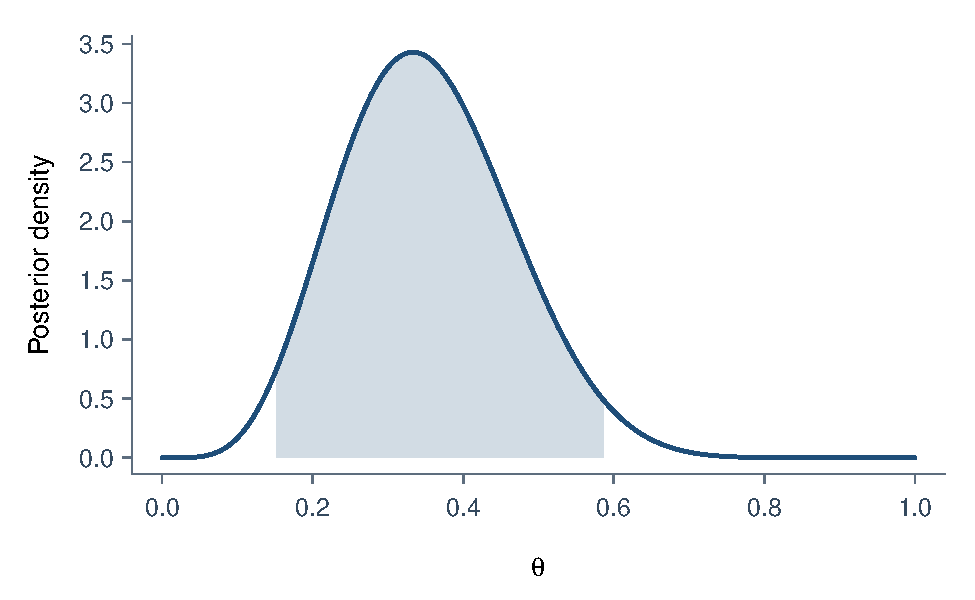
\includegraphics[width=0.68\linewidth]{ex05_negbin.pdf}\end{center}

\begin{answer}
(a) $\theta\mid Y\sim\dist{Beta}(a+m,\,b+Y)$. \quad (b) $\dist{Beta}(6,11)$; 95\% credible interval $(0.152,\ 0.587)$.
\end{answer}

\begin{takeaway}
This is the same posterior as for 5 successes and 10 failures under a \emph{binomial} likelihood: the stopping rule (stop after $m$ successes vs.\ after $n$ trials) does not change Bayesian inference --- the \textbf{likelihood principle}.
\end{takeaway}

% ================================================================= Exercise 6
\exercise{2.6 --- Heart rates and regression to the mean}

\begin{problem}{6}
The distribution of true heart rate across a population is Gaussian with mean 64 beats per minute (bpm) and standard deviation 10 bpm. An individual measurement is unbiased for the true heart rate, but has error standard deviation 5 bpm.
\begin{enumerate}[(a)]
\item Given that an individual has a (single) measured heart rate of $y$ bpm, what is the posterior distribution of their true heart rate? Plot the posterior mean as a function of the observed value and comment on the regression to the mean.
\item Consider a study designed to test a new method to treat high heart rate. To obtain a sample, they measure randomly-selected individuals from the population and include them in the study if and only if their heart rate exceeds 90 bpm. For these individuals, they apply the treatment and measure their heart rate again. The estimate of the treatment effect is the difference in mean heart rate before and after the treatment for the individuals in the study. Assuming the new method has no actual effect on heart rate, compute (using mathematical derivations or simulations) the expected difference in the mean.
\item How could the study in (b) be redesigned to avoid regression to the mean bias?
\end{enumerate}
\end{problem}

\begin{restate}
A noisy measurement of heart rate should be pulled back toward the population average. Show this, then show how it creates a fake ``treatment effect'' in a study that only enrols people with high readings.
\end{restate}

\begin{keyidea}
Normal--normal model with prior $\theta\sim\dist N(64,10^2)$ and $y\mid\theta\sim\dist N(\theta,5^2)$. The posterior mean is $w y+(1-w)64$ with $w=\frac{10^2}{10^2+5^2}=0.8$.
\end{keyidea}

\solution
\step{(a) Posterior.}
Precision: $\frac1{100}+\frac1{25}=0.05\Rightarrow$ variance $20$ (SD 4.47). Mean:
\[
\E(\theta\mid y)=\frac{64/100+y/25}{0.05}=12.8+0.8y,\qquad\theta\mid y\sim\dist{Normal}(12.8+0.8y,\ 20).
\]
\begin{center}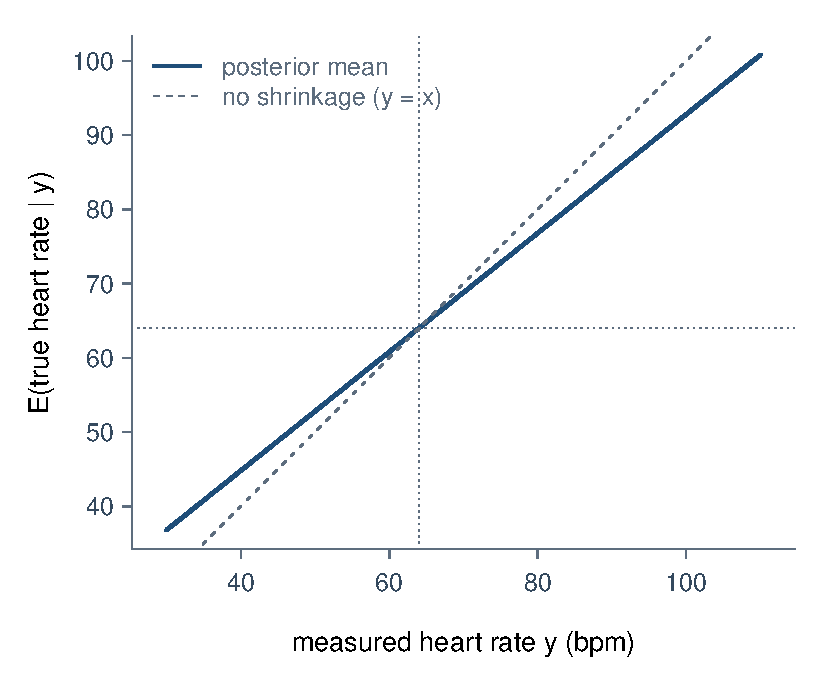
\includegraphics[width=0.55\linewidth]{ex06_shrinkage.pdf}\end{center}
The line has slope $0.8<1$ and crosses the diagonal at 64. A reading of 100 implies a true rate of about 92.8; a reading of 40 implies about 44.8. Extreme readings are partly bad luck in the measurement error, so the best guess \emph{regresses toward the mean}.

\step{(b) The fake effect.}
Let $Y_1=\theta+e_1$ (screening/before) and $Y_2=\theta+e_2$ (after, no treatment effect). Then
\[
\E(Y_1-Y_2\mid Y_1>90)=\E(Y_1\mid Y_1>90)-\E\big(\E(\theta\mid Y_1)\mid Y_1>90\big)=0.2\big(\E(Y_1\mid Y_1>90)-64\big).
\]
Marginally $Y_1\sim\dist N(64,125)$, SD $11.18$. With $z=(90-64)/11.18=2.326$, the truncated-normal mean is
\[
\E(Y_1\mid Y_1>90)=64+11.18\,\frac{\phi(z)}{1-\Phi(z)}=93.79,
\]
so the expected difference is $0.2(93.79-64)=\mathbf{5.96}$ bpm. A simulation of $2\times10^6$ people (20{,}047 enrolled) gives 5.92 bpm.

\step{(c) Redesign.}
\begin{itemize}
\item \textbf{Randomise}: enrol people with $Y_1>90$ and randomly assign half to a placebo/control. Both groups regress to the mean equally; compare their \emph{after} values.
\item Or take a \emph{fresh baseline} measurement after enrolment (independent of the screening value) and compute the change from it.
\item Averaging several screening measurements reduces (but does not remove) the bias.
\end{itemize}

\begin{answer}
(a) $\theta\mid y\sim\dist{Normal}(12.8+0.8y,\ 20)$. \quad (b) $\approx\mathbf{6}$ bpm apparent drop with a useless treatment. \quad (c) Use a randomised control group (or a fresh baseline measurement).
\end{answer}

\begin{takeaway}
Regression to the mean is one of the most common sources of false ``improvements'' in medicine, education and sports. Selecting on an extreme noisy value guarantees the next value is less extreme on average.
\end{takeaway}

% ================================================================= Exercise 7
\exercise{2.7 --- A prior for California wildfires}

\begin{problem}{7}
Over the past 50 years California has experienced an average of $\lambda_0=75$ large wildfires per year. For the next 10 years you will record the number of large fires in California and then fit a Poisson/gamma model to these data. Let the rate of large fires in this future period, $\lambda$, have prior $\lambda\sim\dist{Gamma}(a,b)$. Select $a$ and $b$ so that the prior is uninformative with prior variance around 100 and gives prior probability approximately $\Prob(\lambda>\lambda_0)=0.5$ so that the prior places equal probability on both hypotheses in the test for a change in the rate.
\end{problem}

\begin{restate}
Choose a Gamma prior for the future fire rate whose median is 75 (equal odds of increase or decrease) and whose variance is 100.
\end{restate}

\begin{keyidea}
Two conditions, two unknowns. $\V=a/b^2=100$ gives $b=\sqrt{a}/10$; then solve $\text{median}=75$ numerically (\texttt{uniroot}).
\end{keyidea}

\solution
\step{Quick approximation.} If we set the \emph{mean} to 75: $a/b=75$, $a/b^2=100\Rightarrow b=0.75$, $a=56.25$. But the Gamma is right-skewed, so its median is slightly below its mean: $\Prob(\lambda>75)=0.482$.
\step{Exact.} Solve $\texttt{qgamma}(0.5,\ a,\ \sqrt a/10)=75$: $a=56.91$, $b=0.754$. Check: mean 75.44, SD 10.00, $\Prob(\lambda>75)=0.500$.
\step{Is this ``uninformative''?}
In the Poisson--gamma update $b$ acts like a number of prior \emph{years} of data. Here $b=0.75$, less than one year, while we will collect 10 years. So the data will dominate.

\begin{answer}
$\lambda\sim\dist{Gamma}(a=56.9,\ b=0.754)$: variance 100 (SD 10), median 75. The simpler $\dist{Gamma}(56.25,0.75)$ (mean 75) gives $\Prob(\lambda>75)=0.48$, close enough to ``approximately 0.5''.
\end{answer}

\begin{takeaway}
``Uninformative'' should be judged \emph{relative to the data}: a prior worth 0.75 years is weak against 10 years of counts, even though an SD of 10 fires is not vague in absolute terms.
\end{takeaway}

% ================================================================= Exercise 8
\exercise{2.8 --- Is the measurement error too large?}

\begin{problem}{8}
An assembly line relies on accurate measurements from an image-recognition algorithm at the first stage of the process. It is known that the algorithm is unbiased, so assume that measurements follow a normal distribution with mean zero, $Y_i|\sigma^2\iid\dist{Normal}(0,\sigma^2)$. Some errors are permissible, but if $\sigma$ exceeds the threshold $c$, then the algorithm must be replaced. You make $n=20$ measurements and observe $\sum_{i=1}^nY_i=-2$ and $\sum_{i=1}^nY_i^2=15$ and conduct a Bayesian analysis with $\dist{InvGamma}(a,b)$ prior. Compute the posterior probability that $\sigma>c$ for:
\begin{enumerate}[(a)]
\item $c=1$ and $a=b=0.1$
\item $c=1$ and $a=b=1.0$
\item $c=2$ and $a=b=0.1$
\item $c=2$ and $a=b=1.0$
\end{enumerate}
For each $c$, compute the ratio of probabilities for the two priors (i.e. $a=b=0.1$ and $a=b=1.0$). Which, if any, of the results are sensitive to the prior?
\end{problem}

\begin{restate}
Estimate the error standard deviation from 20 measurements with known mean 0, and compute the probability it exceeds a threshold under two priors.
\end{restate}

\begin{keyidea}
Known mean, unknown variance $\Rightarrow$ \textbf{normal--inverse-gamma}: $\sigma^2\mid\mathbf Y\sim\dist{InvGamma}\big(a+\frac n2,\ b+\frac12\sum Y_i^2\big)$. Since $1/\sigma^2$ is then Gamma, $\Prob(\sigma>c)=\Prob(1/\sigma^2<1/c^2)$ is a Gamma CDF.
\end{keyidea}

\solution
\step{Posterior.}
\[
p(\sigma^2\mid\mathbf Y)\propto(\sigma^2)^{-n/2}e^{-\sum Y_i^2/(2\sigma^2)}\cdot(\sigma^2)^{-a-1}e^{-b/\sigma^2}
\ \Rightarrow\ \sigma^2\mid\mathbf Y\sim\dist{InvGamma}(a+10,\ b+7.5).
\]
$\sum Y_i=-2$ is \emph{not needed}: the mean is known to be 0, so only $\sum Y_i^2$ enters.
\step{Probabilities.} $\Prob(\sigma>c\mid\mathbf Y)=$ \texttt{pgamma(1/c\^{}2, a+10, b+7.5)}.
\begin{center}
\begin{tabular}{c|cc|c}\toprule
 & $a=b=0.1$ & $a=b=1$ & ratio\\\midrule
$c=1$ & 0.2250 & 0.2366 & 0.95\\
$c=2$ & $2.56\times10^{-5}$ & $1.45\times10^{-5}$ & 1.77\\\bottomrule
\end{tabular}
\end{center}

\begin{answer}
(a) 0.225 \quad (b) 0.237 \quad (c) $2.6\times10^{-5}$ \quad (d) $1.4\times10^{-5}$.\\
For $c=1$ the result is \textbf{not} sensitive (ratio 0.95). For $c=2$ the ratio 1.77 shows \textbf{relative} sensitivity in the extreme tail, but both probabilities are negligible, so the \emph{decision} (keep the algorithm) is the same.
\end{answer}

\begin{takeaway}
Tail probabilities far from the data are always the most prior-sensitive quantities, because the likelihood carries almost no information there. Judge sensitivity by whether it changes the decision.
\end{takeaway}

% ================================================================= Exercise 9
\exercise{2.9 --- Induced prior in logistic regression}

\begin{problem}{9}
In simple logistic regression, the probability of a success is regressed onto a single covariate $X$ as
\[
p(X)=\frac{\exp(\alpha+X\beta)}{1+\exp(\alpha+X\beta)}.\qquad(2.51)
\]
Assuming the covariate is distributed as $X\sim\dist{Normal}(0,1)$ and the parameters have priors $\alpha\sim\dist{Normal}(0,c^2)$ and $\beta\sim\dist{Normal}(0,c^2)$, find a prior standard deviation $c$ so that the induced prior on the success probability $p(X)$ is roughly $\dist{Uniform}(0,1)$. That is, for a given $c$ generate $S$ (say $S=1{,}000{,}000$) samples $(X^{(s)},\alpha^{(s)},\beta^{(s)})$ for $s=1,\dots,S$, compute the $S$ success probabilities, and make a histogram of the $S$ probabilities. Repeat this for several $c$ until the histogram is approximately uniform. Report the final value of $c$ and the resulting histogram. Would you call this an uninformative prior for the regression coefficients $\alpha$ and $\beta$?
\end{problem}

\begin{restate}
A prior on the regression coefficients implies a prior on the probability $p(X)$. Find the prior SD $c$ that makes this implied prior flat.
\end{restate}

\begin{keyidea}
If $p\sim\dist{Uniform}(0,1)$ then $\mathrm{logit}(p)$ has a standard logistic distribution with variance $\pi^2/3\approx3.29$. Here $\eta=\alpha+X\beta$ has variance $c^2(1+\E X^2)=2c^2$, so a first guess is $2c^2\approx3.29\Rightarrow c\approx1.28$. Refine by simulation.
\end{keyidea}

\solution
\step{Simulation.} For $c$ from 0.5 to 3 in steps of 0.05, draw $2\times10^5$ triples, compute $p=\mathrm{plogis}(\alpha+X\beta)$, and measure the distance to uniform with the Kolmogorov--Smirnov statistic.
\begin{lstlisting}
induced_p <- function(c, S) plogis(rnorm(S, 0, c) + rnorm(S) * rnorm(S, 0, c))
\end{lstlisting}
The best value is $c=1.30$ (KS distance 0.005 with $S=10^6$).
\begin{center}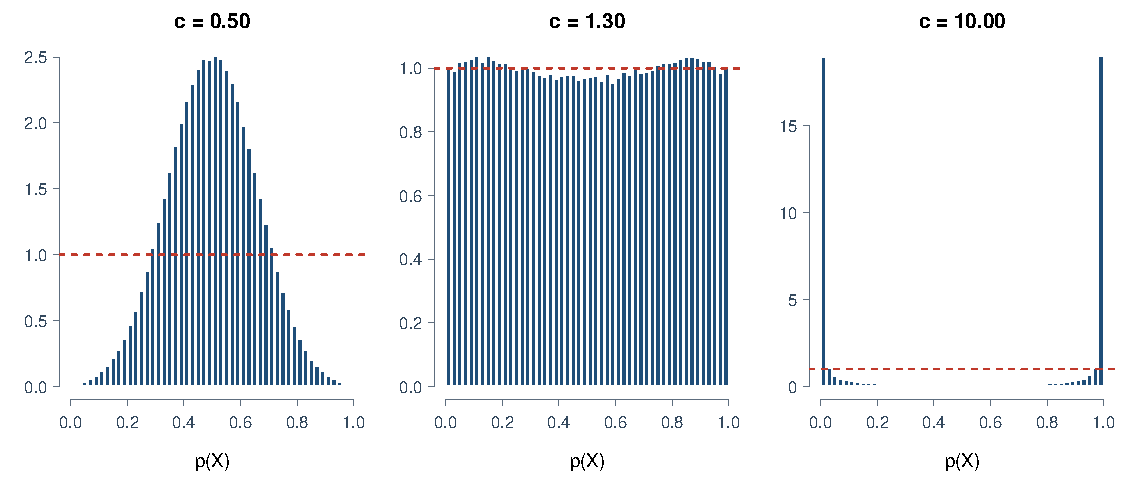
\includegraphics[width=0.98\linewidth]{ex09_induced.pdf}\end{center}
Left: $c=0.5$ concentrates $p$ near 0.5. Middle: $c=1.3$ is flat. Right: the ``vague'' $c=10$ piles almost all mass at $p\approx0$ and $p\approx1$.

\step{Uninformative for $\alpha,\beta$?}
No. $c=1.3$ says that $|\beta|>2.6$ (an odds ratio above $e^{2.6}\approx13$ per SD of $X$) has only about 5\% prior probability --- that is a real, though reasonable, restriction. Conversely, a prior that is vague for the coefficients ($c=10$) is very informative about $p$: it claims success probabilities are almost always near 0 or 1.

\begin{answer}
$c\approx\mathbf{1.3}$ gives an approximately $\dist{Uniform}(0,1)$ induced prior on $p(X)$. It is \textbf{not} uninformative for $\alpha$ and $\beta$; it is a mildly informative prior that is weak on the scale of probabilities.
\end{answer}

\begin{takeaway}
``Uninformative'' depends on the parameterisation. Always check what a prior implies on the scale you care about, a \emph{prior predictive check}.
\end{takeaway}

% ================================================================= Exercise 10
\exercise{2.10 --- Adverse side effects at the Mayo Clinic}

\begin{problem}{10}
The Mayo Clinic conducted a study of $n=50$ patients followed for one year on a new medication and found that 30 patients experienced no adverse side effects (ASE), 12 experienced one ASE, 6 experienced two ASEs and 2 experienced ten ASEs.
\begin{enumerate}[(a)]
\item Derive the posterior of $\lambda$ for the Poisson/gamma model $Y_1,\dots,Y_n|\lambda\iid\dist{Poisson}(\lambda)$ and $\lambda\sim\dist{Gamma}(a,b)$.
\item Use the Poisson/gamma model with $a=b=0.01$ to study the rate of adverse events. Plot the posterior and give the posterior mean and 95\% credible interval.
\item Repeat this analysis with $\dist{Gamma}(0.1,0.1)$ and $\dist{Gamma}(1,1)$ priors and discuss sensitivity to the prior.
\item Plot the data versus the $\dist{Poisson}(\hat\lambda)$ PMF, where $\hat\lambda$ is the posterior mean of $\lambda$ from part (b). Does the Poisson likelihood fit well?
\item The current medication is thought to have around one adverse side effect per year. What is the posterior probability that this new medication has a higher side effect rate than the previous medication? Are the results sensitive to the prior?
\end{enumerate}
\end{problem}

\begin{restate}
Estimate the yearly rate of side effects from 50 patients, check prior sensitivity and model fit, and compare with a rate of 1 per year.
\end{restate}

\begin{keyidea}
Poisson--gamma conjugacy as in Exercise 2.2. For model checking, compare the observed frequency of each count with the Poisson probabilities. For a Poisson, variance $=$ mean.
\end{keyidea}

\solution
\step{(a)}
\[
p(\lambda\mid\mathbf Y)\propto\prod_i\lambda^{Y_i}e^{-\lambda}\cdot\lambda^{a-1}e^{-b\lambda}=\lambda^{a+\sum Y_i-1}e^{-(b+n)\lambda}\ \Rightarrow\ \lambda\mid\mathbf Y\sim\dist{Gamma}\Big(a+\sum Y_i,\ b+n\Big).
\]
\step{(b)} $\sum Y_i=0(30)+1(12)+2(6)+10(2)=44$, $n=50$: $\lambda\mid\mathbf Y\sim\dist{Gamma}(44.01,\ 50.01)$, mean $0.880$, 95\% interval $(0.639,\ 1.158)$.
\begin{center}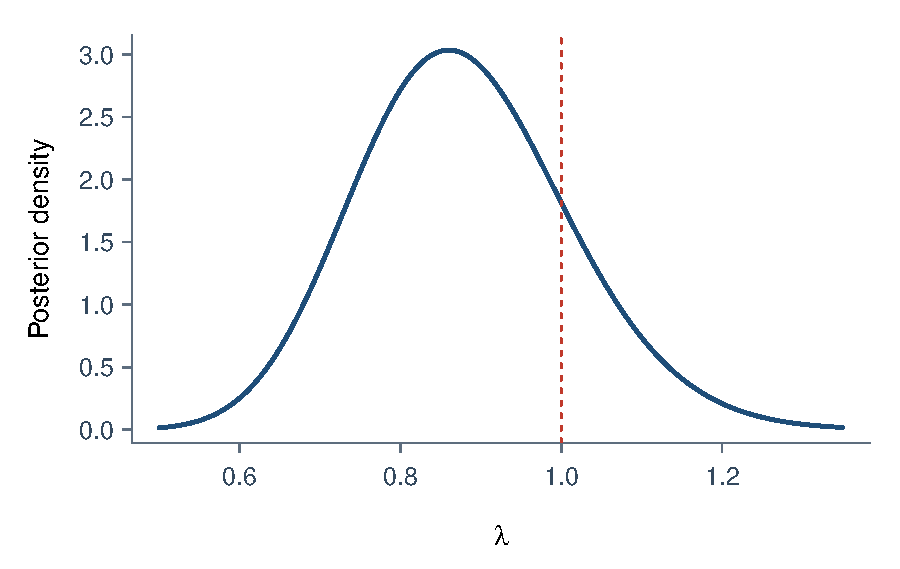
\includegraphics[width=0.66\linewidth]{ex10_posterior.pdf}\end{center}
\step{(c) Sensitivity.}
\begin{center}
\begin{tabular}{lcccc}\toprule
Prior & Posterior & Mean & 95\% interval & $\Prob(\lambda>1)$\\\midrule
$\dist{Gamma}(0.01,0.01)$ & $\dist{Gamma}(44.01,50.01)$ & 0.880 & (0.639, 1.158) & 0.180\\
$\dist{Gamma}(0.1,0.1)$ & $\dist{Gamma}(44.1,50.1)$ & 0.880 & (0.640, 1.158) & 0.180\\
$\dist{Gamma}(1,1)$ & $\dist{Gamma}(45,51)$ & 0.882 & (0.644, 1.158) & 0.182\\\bottomrule
\end{tabular}
\end{center}
Essentially no sensitivity: 44 events and 50 patient-years swamp priors worth at most 1 event and 1 year.

\step{(d) Fit.}
\begin{center}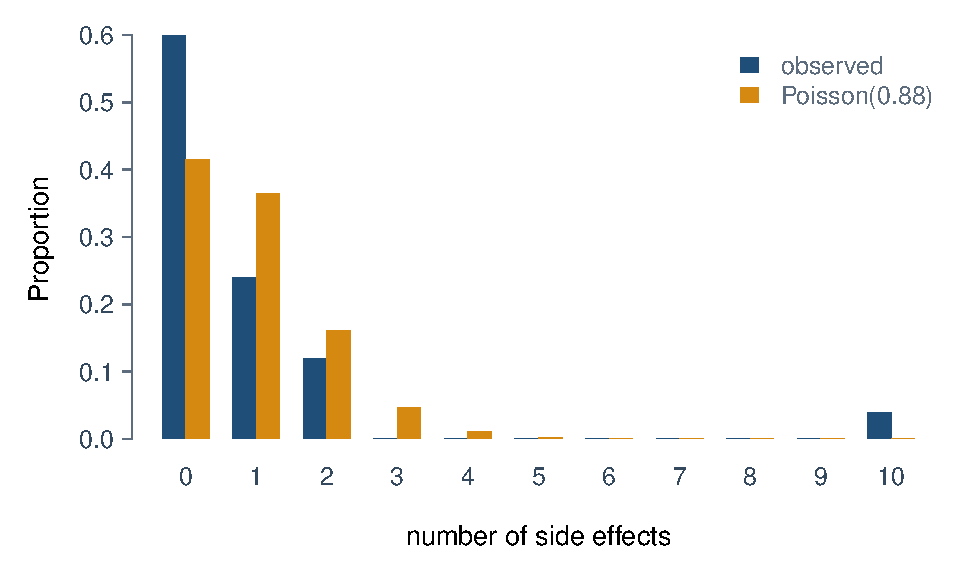
\includegraphics[width=0.75\linewidth]{ex10_fit.pdf}\end{center}
The fit is \textbf{poor}. The Poisson(0.88) predicts 20.7 patients with zero events (observed 30), and $\Prob(Y\ge10)=3.5\times10^{-8}$, yet 2 of 50 patients had ten. The sample variance (4.03) is about 4.6 times the mean (0.88): strong \textbf{over-dispersion}.

\step{(e)} $\Prob(\lambda>1\mid\mathbf Y)\approx0.18$ under all three priors, so it is not sensitive to the prior.

\begin{answer}
(a) $\dist{Gamma}(a+\sum Y_i,\ b+n)$. \quad (b) $\dist{Gamma}(44.01,50.01)$: mean 0.88, 95\% CI $(0.64,1.16)$. \quad (c) Insensitive.\\
(d) Poor fit: too many zeros and two extreme patients (over-dispersion). \quad (e) $\Prob(\lambda>1\mid\mathbf Y)\approx0.18$, insensitive to the prior --- but \emph{sensitive to the model}.
\end{answer}

\begin{takeaway}
Prior sensitivity and model sensitivity are different things. Here the prior does not matter, but the Poisson model is wrong and makes the interval far too narrow. A negative binomial (or a patient-level random effect) would be more honest.
\end{takeaway}

% ================================================================= Exercise 11
\exercise{2.11 --- Days until a smoker relapses}

\begin{problem}{11}
A smoker is trying to quit and their goal is to abstain for one week because studies have shown that this is the most difficult period. Denote $Y$ as the number of days before the smoker relapses, and $\theta$ as the probability that they relapse on any given day of the study.
\begin{enumerate}[(a)]
\item Argue that a negative binomial distribution (Appendix A.1) for $Y|\theta$ is reasonable. What are the most important assumptions being made, and are they valid for this smoking cessation attempt?
\item Assuming a negative binomial likelihood and $\dist{Uniform}(0,1)$ prior for $\theta$, what is the prior probability the smoker will be smoke-free for at least 7 days?
\item Plot the posterior distribution of $\theta$ assuming $Y=5$.
\item Given this attempt resulted in $Y=5$ and that $\theta$ is the same in the second attempt, what is the posterior predictive probability the second attempt will result in at least 7 smoke-free days?
\end{enumerate}
\end{problem}

\begin{restate}
Each day the smoker relapses with probability $\theta$. Model the number of smoke-free days, then update with an attempt that lasted 5 days and predict the next attempt.
\end{restate}

\begin{keyidea}
Each day is a Bernoulli trial: ``relapse'' $=$ success with probability $\theta$. $Y=$ number of failures (smoke-free days) before the first success, so $Y\mid\theta\sim\dist{NegBinomial}(\theta,1)=\dist{Geometric}(\theta)$: $\Prob(Y=y\mid\theta)=\theta(1-\theta)^y$ and $\Prob(Y\ge k\mid\theta)=(1-\theta)^k$.
\end{keyidea}

\solution
\step{(a) Justification and assumptions.}
Counting days until the first ``event'' in a sequence of trials is exactly the negative binomial with $m=1$. It assumes:
\begin{enumerate}[(i)]
\item the relapse probability $\theta$ is the \textbf{same every day} --- questionable: cravings are strongest in the first few days, so the daily risk likely \emph{decreases} over time;
\item days are \textbf{independent} --- questionable: a stressful day raises the next day's risk too;
\item time is measured in whole days.
\end{enumerate}
Still, it is a reasonable first approximation.

\step{(b) Prior probability of $\ge7$ days.}
\[
\Prob(Y\ge7)=\int_0^1(1-\theta)^7\cdot1\dd\theta=\frac18=0.125.
\]

\step{(c) Posterior with $Y=5$.}
$p(\theta\mid Y=5)\propto\theta(1-\theta)^5\Rightarrow\theta\mid Y\sim\dist{Beta}(2,6)$: mean 0.25, 95\% interval $(0.037,\ 0.579)$.
\begin{center}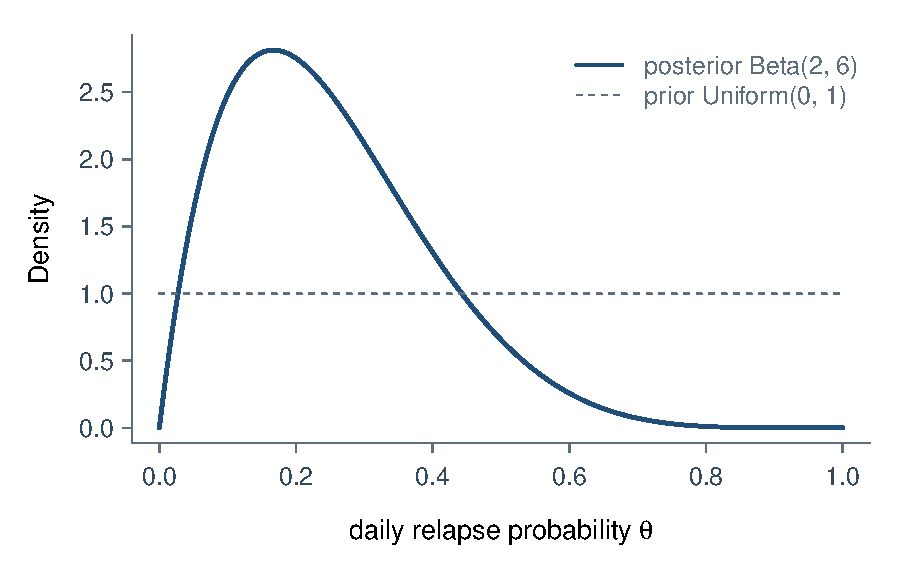
\includegraphics[width=0.66\linewidth]{ex11_posterior.pdf}\end{center}

\step{(d) Posterior predictive.}
\[
\Prob(Y^*\ge7\mid Y=5)=\E\big[(1-\theta)^7\mid Y\big]=\frac{B(2,13)}{B(2,6)}=\frac{1!\,12!/14!}{1!\,5!/7!}=\frac{6\cdot7}{13\cdot14}=\frac{3}{13}\approx0.231.
\]
Monte Carlo check (draw $\theta$, then $Y^*$): 0.2307.

\begin{answer}
(a) Geometric $=\dist{NegBinomial}(\theta,1)$; it assumes a constant, independent daily relapse risk (doubtful). \quad (b) $1/8=0.125$. \quad (c) $\dist{Beta}(2,6)$. \quad (d) $3/13\approx\mathbf{0.231}$.
\end{answer}

\begin{takeaway}
The previous attempt (5 days) is informative: the chance of reaching a week rises from 12.5\% to 23\%. Integrate over the posterior; plugging in $\hat\theta=0.25$ would give $0.75^7=0.133$, understating the chance because it ignores the possibility of a small $\theta$.
\end{takeaway}

% ================================================================= Exercise 12
\exercise{2.12 --- Censored relapse times}

\begin{problem}{12}
A smoking cessation study followed $n=20$ patients until they relapsed to smoking. The trial terminated after six weeks and so many patients did not relapse during the observation period; i.e., their responses was censored. Seven patients relapsed during the observation period at times 0.5, 0.9, 1.1, 2.4, 3.8, 4.0 and 5.2 weeks, and the rest were censored at 6 weeks. Assume the times to event $Y_1,\dots,Y_n$ follow the survival analysis model $Y_i|\lambda\iid\dist{Exponential}(\lambda)$ with prior $\lambda\sim\dist{Gamma}(a,b)$.
\begin{enumerate}[(a)]
\item Show that the posterior distribution of $\lambda$ is a gamma distribution (hint: the likelihood contribution of a censored observation is $\Prob(Y_i>6|\lambda)=\exp(-6\lambda)$).
\item Compute the posterior mean and 95\% interval for $\lambda$ for several values of $a$ and $b$. Are the results sensitive to the prior?
\end{enumerate}
\end{problem}

\begin{restate}
Seven patients relapsed at known times; thirteen were still smoke-free when the study ended. Use both kinds of information to estimate the relapse rate.
\end{restate}

\begin{keyidea}
Observed event at $y$: contributes the density $\lambda e^{-\lambda y}$. Censored at 6: contributes the survival probability $e^{-6\lambda}$. The posterior depends only on the number of events $d$ and the total time at risk $T$.
\end{keyidea}

\solution
\step{(a) Likelihood and posterior.}
\[
L(\lambda)=\prod_{i=1}^{7}\lambda e^{-\lambda y_i}\times\prod_{j=1}^{13}e^{-6\lambda}=\lambda^{7}\exp\{-\lambda(17.9+78)\}=\lambda^{d}e^{-\lambda T},
\]
with $d=7$ events and $T=0.5+0.9+1.1+2.4+3.8+4.0+5.2+13\times6=95.9$ patient-weeks. With the $\dist{Gamma}(a,b)$ prior,
\[
p(\lambda\mid\text{data})\propto\lambda^{a+d-1}e^{-(b+T)\lambda}\ \Rightarrow\ \lambda\mid\text{data}\sim\dist{Gamma}(a+7,\ b+95.9).
\]
\step{(b) Several priors.}
\begin{center}
\begin{tabular}{lccc}\toprule
Prior & Posterior & Mean (per week) & 95\% interval\\\midrule
$\dist{Gamma}(0.01,0.01)$ & $\dist{Gamma}(7.01,95.91)$ & 0.073 & (0.029, 0.136)\\
$\dist{Gamma}(0.1,0.1)$ & $\dist{Gamma}(7.1,96.0)$ & 0.074 & (0.030, 0.138)\\
$\dist{Gamma}(1,1)$ & $\dist{Gamma}(8,96.9)$ & 0.083 & (0.036, 0.149)\\
$\dist{Gamma}(2,10)$ & $\dist{Gamma}(9,105.9)$ & 0.085 & (0.039, 0.149)\\\bottomrule
\end{tabular}
\end{center}
The vague priors agree closely. Priors that add one or two pseudo-events shift the mean by about 15\%, which is noticeable because there are only 7 events.

\begin{answer}
(a) $\lambda\mid\text{data}\sim\dist{Gamma}(a+7,\ b+95.9)$. \quad (b) With vague priors, mean $\approx0.073$ relapses/week (mean time to relapse $\approx14$ weeks), 95\% CI $\approx(0.03,0.14)$. Results are mildly sensitive because there are only 7 events.
\end{answer}

\begin{takeaway}
\textbf{Never drop censored observations.} Using only the 7 relapse times gives a rate of $1/2.56=0.39$ per week --- five times too high --- because the 13 patients who did well are thrown away. They contribute 78 of the 95.9 weeks at risk.
\end{takeaway}

% ================================================================= Exercise 13
\exercise{2.13 --- Mixture-of-experts prior for an alarm}

\begin{problem}{13}
You are designing a very small experiment to determine the sensitivity of a new security alarm system. You will simulate five robbery attempts and record the number of these attempts that trigger the alarm. Because the dataset will be small, you ask two experts for their opinion. One expects the alarm probability to be 0.95 with standard deviation 0.05, and the other expects 0.80 with standard deviation 0.20.
\begin{enumerate}[(a)]
\item Translate these two priors into beta PDFs, and plot the two beta PDFs and the corresponding mixture of experts prior with equal weight given to each expert.
\item Now you conduct the experiment, and the alarm is triggered in every simulated robbery. Plot the posterior of the alarm probability under a uniform prior, each experts' prior, and the mixture of experts prior.
\end{enumerate}
\end{problem}

\begin{restate}
Turn two experts' (mean, SD) opinions into beta priors, average them, and update all priors with 5 alarms out of 5 attempts.
\end{restate}

\begin{keyidea}
\textbf{Beta moment matching}: for mean $\mu$ and variance $v$, $a+b=\frac{\mu(1-\mu)}{v}-1$, $a=\mu(a+b)$, $b=(1-\mu)(a+b)$.
\textbf{Mixture update}: a mixture of conjugate priors gives a mixture of the conjugate posteriors, with weights $\propto$ prior weight $\times$ marginal likelihood $\frac{B(a_k+Y,\,b_k+n-Y)}{B(a_k,b_k)}$.
\end{keyidea}

\solution
\step{(a) The two priors.}
Expert 1: $\frac{0.95\cdot0.05}{0.0025}-1=18\Rightarrow\dist{Beta}(17.1,\ 0.9)$.
Expert 2: $\frac{0.8\cdot0.2}{0.04}-1=3\Rightarrow\dist{Beta}(2.4,\ 0.6)$.
Mixture: $\pi(\theta)=0.5\,\dist{Beta}(\theta;17.1,0.9)+0.5\,\dist{Beta}(\theta;2.4,0.6)$.
\begin{center}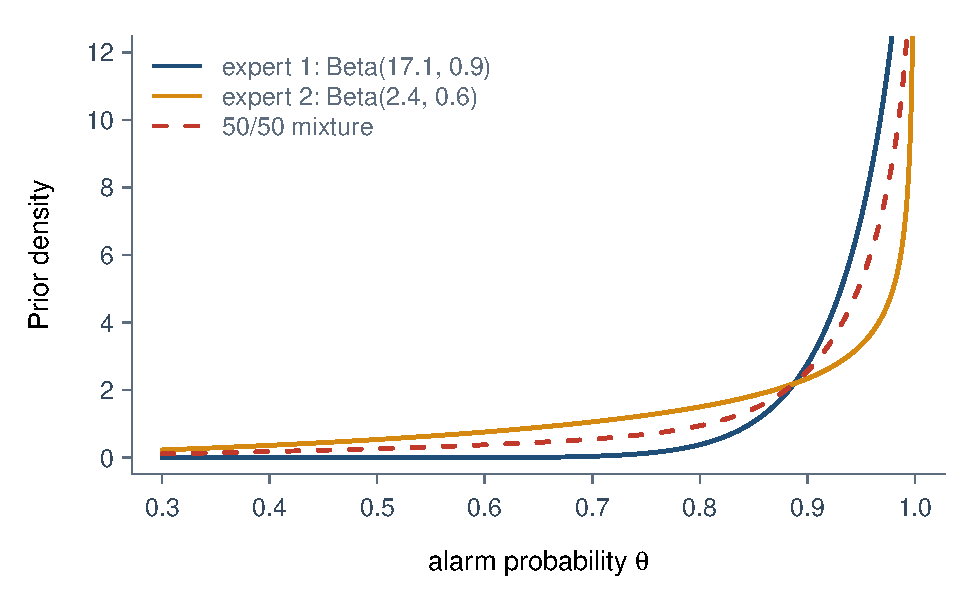
\includegraphics[width=0.72\linewidth]{ex13_priors.pdf}\end{center}

\step{(b) Posteriors after $Y=5$ of $n=5$.}
\begin{itemize}
\item Uniform: $\dist{Beta}(6,1)$, mean 0.857.
\item Expert 1: $\dist{Beta}(22.1,0.9)$, mean 0.961.
\item Expert 2: $\dist{Beta}(7.4,0.6)$, mean 0.925.
\item Mixture: new weights $\propto0.5\,\frac{B(22.1,0.9)}{B(17.1,0.9)}$ and $0.5\,\frac{B(7.4,0.6)}{B(2.4,0.6)}$, which normalise to $\mathbf{0.617}$ and $\mathbf{0.383}$. Mean $0.617(0.961)+0.383(0.925)=0.947$.
\end{itemize}
\begin{center}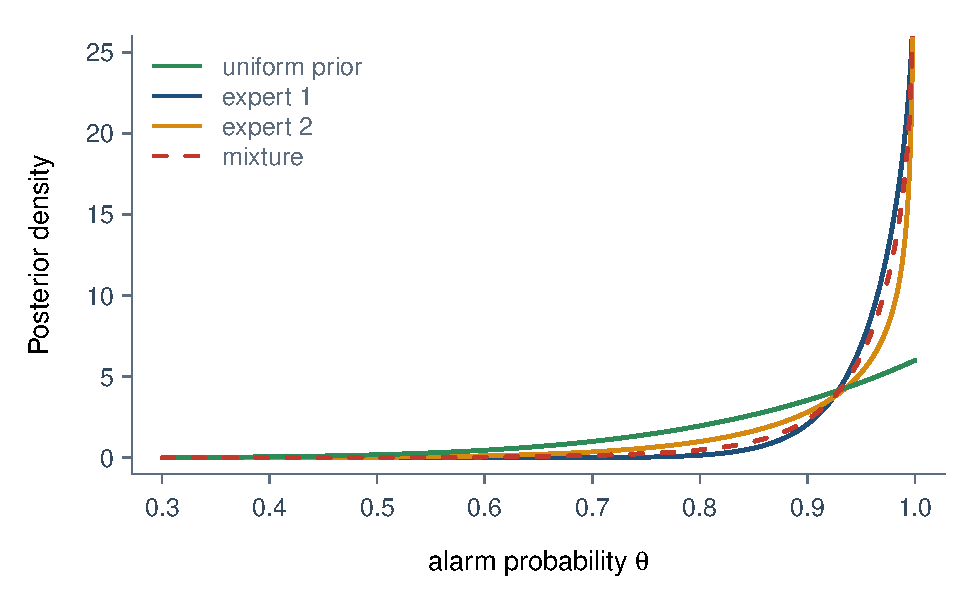
\includegraphics[width=0.72\linewidth]{ex13_posteriors.pdf}\end{center}

\begin{answer}
(a) Expert 1 $=\dist{Beta}(17.1,0.9)$, expert 2 $=\dist{Beta}(2.4,0.6)$, mixture $=$ their 50/50 average.\\
(b) Posteriors: uniform $\dist{Beta}(6,1)$; expert 1 $\dist{Beta}(22.1,0.9)$; expert 2 $\dist{Beta}(7.4,0.6)$; mixture $0.617\,\dist{Beta}(22.1,0.9)+0.383\,\dist{Beta}(7.4,0.6)$ (mean 0.947).
\end{answer}

\begin{takeaway}
The data (5/5) favour the more optimistic expert, so the posterior shifts weight toward expert 1 (from 50\% to 62\%). A mixture prior is a principled way to combine disagreeing experts --- the data decide whom to trust.
\end{takeaway}

% ================================================================= Exercise 14
\exercise{2.14 --- Probability or odds: which scale is ``flat''?}

\begin{problem}{14}
Let $\theta$ be the binomial success probability and $\gamma=\theta/(1-\theta)$ be the corresponding odds of a success. Use Monte Carlo simulation (you can discard samples with $\gamma>100$) to explore the effects of parameterization on prior choice in this context.
\begin{enumerate}[(a)]
\item If $\theta\sim\dist{Uniform}(0,1)$, what is the induced prior on $\gamma$?
\item If $\theta\sim\dist{Beta}(0.5,0.5)$, what is the induced prior on $\gamma$?
\item If $\gamma\sim\dist{Uniform}(0,100)$, what is the induced prior on $\theta$?
\item If $\gamma\sim\dist{Gamma}(1,1)$, what is the induced prior on $\theta$?
\item Would you say any of these priors are simultaneously uninformative for both $\theta$ and $\gamma$?
\end{enumerate}
\end{problem}

\begin{restate}
Put a prior on the probability $\theta$ and see what it says about the odds $\gamma$, and vice versa.
\end{restate}

\begin{keyidea}
\textbf{Change of variables}: if $\gamma=g(\theta)$ is monotone, $f_\gamma(\gamma)=f_\theta\big(g^{-1}(\gamma)\big)\,\big|\frac{\dd\theta}{\dd\gamma}\big|$. Here $\theta=\frac{\gamma}{1+\gamma}$ and $\frac{\dd\theta}{\dd\gamma}=\frac1{(1+\gamma)^2}$; conversely $\frac{\dd\gamma}{\dd\theta}=\frac{1}{(1-\theta)^2}$. Monte Carlo: just transform the draws.
\end{keyidea}

\solution
\step{(a)} $f(\gamma)=1\cdot\frac1{(1+\gamma)^2}$, $\gamma>0$. Decreasing, with median 1 but a heavy tail ($\E\gamma=\infty$).
\step{(b)} $f(\gamma)=\frac{1}{\pi}\theta^{-1/2}(1-\theta)^{-1/2}\frac{1}{(1+\gamma)^2}=\frac{1}{\pi\sqrt\gamma\,(1+\gamma)}$. It has an infinite spike at $\gamma=0$ and a heavy tail.
\step{(c)} $f(\theta)=\frac1{100}\cdot\frac1{(1-\theta)^2}$ for $0<\theta<\frac{100}{101}$. Almost all mass is near 1: $\Prob(\theta>0.9)=\Prob(\gamma>9)=0.91$.
\step{(d)} $f(\theta)=\exp\!\big(-\tfrac{\theta}{1-\theta}\big)\frac{1}{(1-\theta)^2}$, $0<\theta<1$. Hump-shaped around 0.5 and falling to 0 near 1 ($\Prob(\theta>0.9)=e^{-9}\approx0.0001$).

Simulated histograms ($10^6$ draws, $\gamma>100$ discarded) with the exact densities in red:
\begin{center}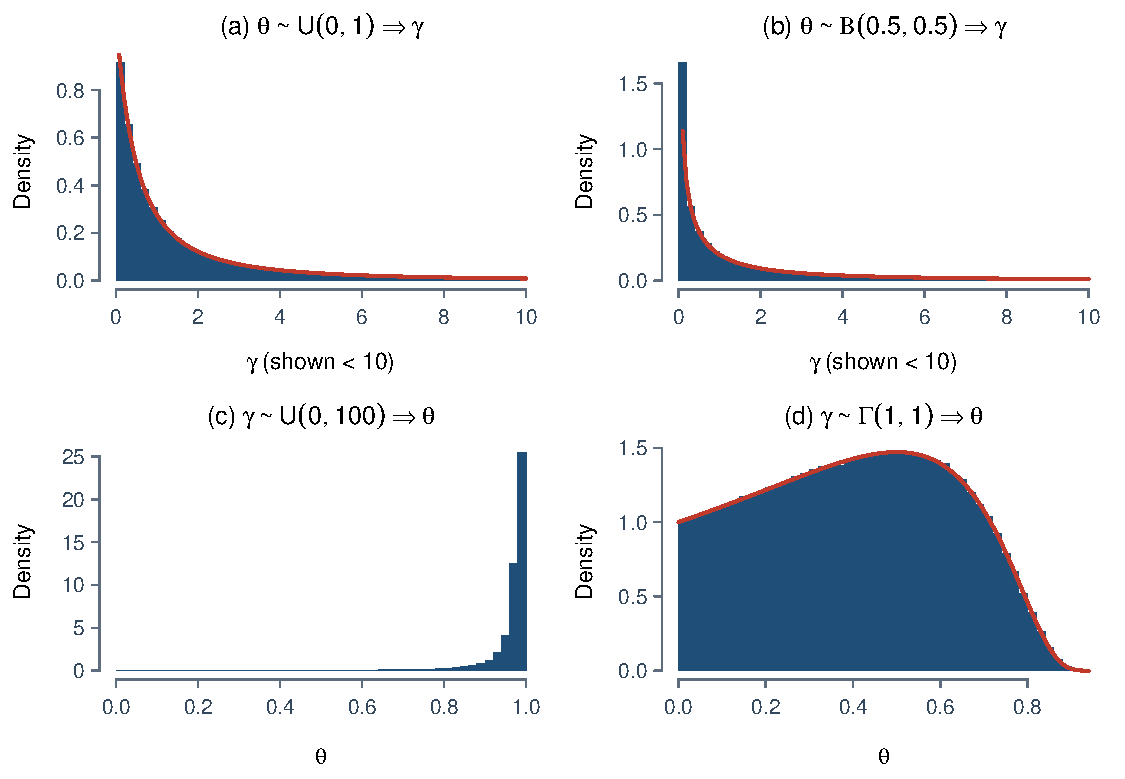
\includegraphics[width=0.95\linewidth]{ex14_reparam.pdf}\end{center}

\step{(e)} None of them is flat on both scales. A uniform $\theta$ gives a strongly skewed prior on $\gamma$; a uniform $\gamma$ pushes $\theta$ toward 1. Because the transformation is nonlinear, ``flat'' on one scale means ``non-flat'' on the other.

\begin{answer}
(a) $\frac1{(1+\gamma)^2}$ \quad (b) $\frac1{\pi\sqrt\gamma(1+\gamma)}$ \quad (c) $\frac{1}{100(1-\theta)^2}$ on $(0,\frac{100}{101})$ \quad (d) $\frac{e^{-\theta/(1-\theta)}}{(1-\theta)^2}$\\
(e) \textbf{No} prior is uninformative on both scales simultaneously.
\end{answer}

\begin{takeaway}
This is exactly the problem the \textbf{Jeffreys prior} solves: it is not flat, but it gives the \emph{same} answer whichever parameterisation you start from. The $\dist{Beta}(0.5,0.5)$ in (b) is the Jeffreys prior for the binomial.
\end{takeaway}

% ================================================================= Exercise 15
\exercise{2.15 --- A flat prior can give a proper posterior}

\begin{problem}{15}
Say $Y|\mu\sim\dist{Normal}(\mu,1)$ and $\mu$ has improper prior $\pi(\mu)=1$ for all $\mu$. Prove that the posterior distribution of $\mu$ is a proper PDF.
\end{problem}

\begin{restate}
Even though the flat prior does not integrate to 1, show that the posterior does.
\end{restate}

\begin{keyidea}
A posterior is proper iff the marginal $m(Y)=\int f(Y\mid\mu)\pi(\mu)\dd\mu$ is finite.
\end{keyidea}

\solution
\step{Marginal.}
\[
m(Y)=\int_{-\infty}^{\infty}\frac{1}{\sqrt{2\pi}}e^{-(Y-\mu)^2/2}\cdot1\dd\mu=1<\infty,
\]
because, as a function of $\mu$, the integrand is the $\dist{Normal}(Y,1)$ density.
\step{Posterior.}
\[
p(\mu\mid Y)=\frac{f(Y\mid\mu)\pi(\mu)}{m(Y)}=\frac{1}{\sqrt{2\pi}}e^{-(\mu-Y)^2/2},
\]
which is non-negative and integrates to 1.

\begin{answer}
$p(\mu\mid Y)\propto e^{-(\mu-Y)^2/2}$ has finite integral $\sqrt{2\pi}$, so the posterior is the proper density $\mu\mid Y\sim\dist{Normal}(Y,1)$.
\end{answer}

\begin{takeaway}
An improper prior is acceptable only if the posterior is proper, and this must be \emph{checked} for each model (see Exercises 16--17 for cases where it fails).
\end{takeaway}

% ================================================================= Exercise 16
\exercise{2.16 --- When an improper prior must fail}

\begin{problem}{16}
Suppose that the likelihood $f(\mathbf Y|\theta)\ge c(\mathbf Y)$ for all $\theta$. Show that an improper prior on $\theta$ will yield an improper posterior.
\end{problem}

\begin{restate}
If the likelihood never drops below some positive level, the data cannot ``tame'' an infinite prior.
\end{restate}

\begin{keyidea}
Improper prior: $\int\pi(\theta)\dd\theta=\infty$. The posterior is proper iff $m(\mathbf Y)=\int f(\mathbf Y\mid\theta)\pi(\theta)\dd\theta<\infty$.
\end{keyidea}

\solution
Assume $c(\mathbf Y)>0$ (otherwise the bound says nothing). Then, since $\pi\ge0$,
\[
m(\mathbf Y)=\int f(\mathbf Y\mid\theta)\pi(\theta)\dd\theta\ \ge\ \int c(\mathbf Y)\pi(\theta)\dd\theta=c(\mathbf Y)\int\pi(\theta)\dd\theta=\infty.
\]
So the normalising constant is infinite and $f(\mathbf Y\mid\theta)\pi(\theta)$ cannot be normalised into a density: the posterior is improper.

\begin{answer}
$m(\mathbf Y)\ge c(\mathbf Y)\int\pi(\theta)\dd\theta=\infty$ whenever $c(\mathbf Y)>0$, so the posterior is improper.
\end{answer}

\begin{takeaway}
For a proper posterior with an improper prior, the likelihood must \emph{decay} in the directions where the prior has infinite mass.
\end{takeaway}

% ================================================================= Exercise 17
\exercise{2.17 --- Mixture models and improper priors}

\begin{problem}{17}
Consider a sample of size $n$ from the mixture of two normal densities given by $f(y|\theta)=0.5\phi(y)+0.5\phi(y-\theta)$ where $\phi(z)$ denotes the standard normal density function. Show that any improper prior for $\theta$ leads to an improper posterior.
\end{problem}

\begin{restate}
Half the data come from $\dist N(0,1)$ and half from $\dist N(\theta,1)$. Show that no improper prior on $\theta$ can work.
\end{restate}

\begin{keyidea}
Find a lower bound for the likelihood that does not depend on $\theta$, then apply Exercise 16.
\end{keyidea}

\solution
\step{Lower bound.} Since $\phi(y_i-\theta)\ge0$,
\[
f(y_i\mid\theta)=0.5\phi(y_i)+0.5\phi(y_i-\theta)\ \ge\ 0.5\phi(y_i)\quad\text{for all }\theta.
\]
\step{For the whole sample.} By independence,
\[
f(\mathbf y\mid\theta)=\prod_{i=1}^n f(y_i\mid\theta)\ \ge\ \prod_{i=1}^n0.5\phi(y_i)=:c(\mathbf y)>0,
\]
because $\phi>0$ everywhere.
\step{Conclude.} By Exercise 16, $m(\mathbf y)\ge c(\mathbf y)\int\pi(\theta)\dd\theta=\infty$.

\begin{answer}
$f(\mathbf y\mid\theta)\ge\prod_i0.5\phi(y_i)>0$ for all $\theta$, so by Exercise 16 every improper prior gives an improper posterior.
\end{answer}

\begin{takeaway}
Intuition: as $\theta\to\pm\infty$ the likelihood does not go to 0 --- it is always possible that every observation came from the first component, which says nothing about $\theta$. Mixture models need proper priors.
\end{takeaway}

% ================================================================= Exercise 18
\exercise{2.18 --- An evidence-based prior for clinical trials}

\begin{problem}{18}
Say a randomized clinical trial is conducted to compare the difference in the mean response between two treatment groups. The effect size $b$ is estimated as the difference between the sample means of the two groups, and $b$ has standard error $s$, and thus the z-score is $z=b/s$. The true difference between treatment group means is $\beta$, and the signal-to-noise ratio is $\delta=\beta/s$. We fit the model $z|\delta\sim\dist{Normal}(\delta,1)$ and $\delta$ has mixture prior in (2.33).
\begin{enumerate}[(a)]
\item Plot the posterior distribution of $\delta$ if we observe $z=2$.
\item Compute the posterior probability that $\delta>0$ given $z=2$.
\item Compute the posterior probability that $\delta>0$ for value of $z\in\{0.0,0.1,\dots,5.0\}$ and plot the probabilities by $z$.
\item Repeat these analyses using prior $\delta\sim\dist{Normal}(0,100^2)$, and comment on the effect of the prior.
\end{enumerate}
\end{problem}

\begin{restate}
Using a prior learned from 20{,}000 real trials, update the true signal-to-noise ratio $\delta$ after seeing $z$, and compare with a nearly flat prior.
\end{restate}

\begin{keyidea}
Prior (2.33) is a mixture of four zero-mean normals:
\[
\pi(\delta)=\sum_{k=1}^4w_k\,\phi(\delta;0,\tau_k^2),\qquad w=(0.32,\,0.31,\,0.30,\,0.07),\quad \tau=(1.17,\,1.74,\,2.38,\,5.73).
\]
For one component, $z\mid\delta\sim\dist N(\delta,1)$ and $\delta\sim\dist N(0,\tau^2)$ give
\[
\delta\mid z\sim\dist N\Big(\tfrac{\tau^2}{1+\tau^2}z,\ \tfrac{\tau^2}{1+\tau^2}\Big),\qquad z\sim\dist N(0,1+\tau^2)\text{ marginally}.
\]
For the mixture, the posterior is a mixture of these, with weights $w_k'\propto w_k\,\phi(z;0,1+\tau_k^2)$.
\end{keyidea}

\solution
\step{(a) Posterior for $z=2$.}
\begin{center}
\begin{tabular}{lcccc}\toprule
Component & 1 & 2 & 3 & 4\\\midrule
prior weight $w_k$ & 0.32 & 0.31 & 0.30 & 0.07\\
posterior weight $w'_k$ & 0.318 & 0.335 & 0.307 & 0.040\\
shrinkage $\tau_k^2/(1+\tau_k^2)$ & 0.578 & 0.752 & 0.850 & 0.970\\
component mean & 1.156 & 1.503 & 1.700 & 1.941\\\bottomrule
\end{tabular}
\end{center}
Posterior mean $\sum w'_k\cdot\text{mean}_k=1.47$.
\begin{center}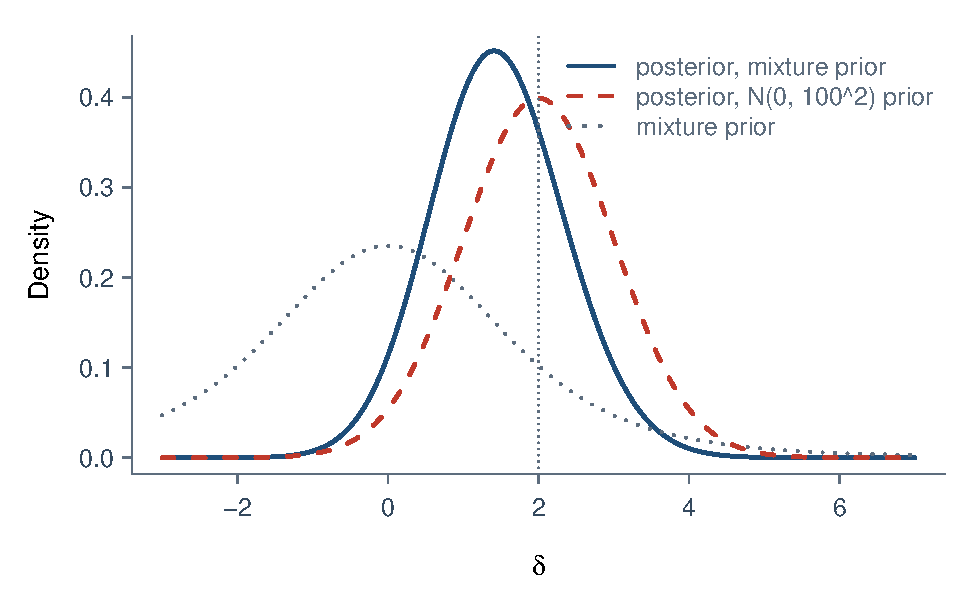
\includegraphics[width=0.72\linewidth]{ex18_posterior.pdf}\end{center}
\step{(b)} $\Prob(\delta>0\mid z=2)=\sum_kw'_k\,\Phi\big(\text{mean}_k/\text{sd}_k\big)=\mathbf{0.955}$.
\step{(c) Across $z$.}
\begin{center}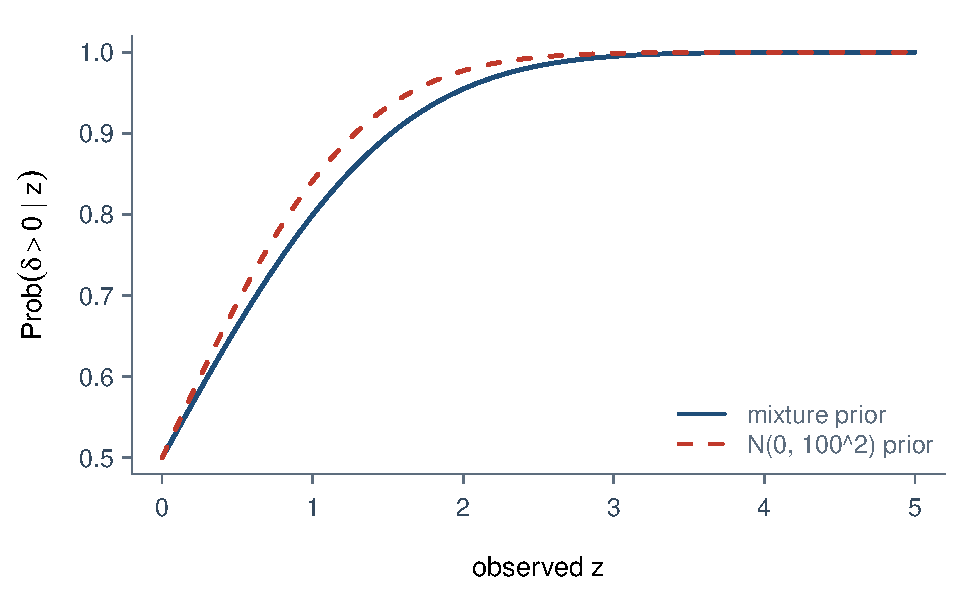
\includegraphics[width=0.68\linewidth]{ex18_pz.pdf}\end{center}
\step{(d) Vague prior $\dist N(0,100^2)$.}
Shrinkage $10^4/(1+10^4)\approx1$, so $\delta\mid z\approx\dist N(z,1)$, posterior mean 2.00 and $\Prob(\delta>0\mid z=2)=\Phi(2)=0.977$ (dashed curves above).
\begin{center}
\begin{tabular}{lccccc}\toprule
$z$ & 1 & 1.96 & 2 & 3 & 4\\\midrule
mixture prior & 0.800 & 0.951 & 0.955 & 0.995 & 0.9997\\
$\dist N(0,100^2)$ prior & 0.841 & 0.975 & 0.977 & 0.999 & 1.000\\\bottomrule
\end{tabular}
\end{center}

\begin{answer}
(a) A four-component normal mixture centred at 1.47 (vs.\ the observed $z=2$). \quad (b) $\Prob(\delta>0\mid z=2)=0.955$.\\
(c) Increases from 0.5 at $z=0$ to essentially 1 by $z\approx4$. \quad (d) The vague prior gives $\delta\mid z\approx\dist N(z,1)$ and $\Prob(\delta>0\mid z=2)=0.977$, i.e.\ \emph{no shrinkage}; the empirical prior shrinks the estimate by about 25\% and is less confident.
\end{answer}

\begin{takeaway}
The evidence-based prior corrects the ``winner's curse'': a trial that just reaches significance ($z\approx2$) usually overestimates the true effect, because most real effects are small. Notice that $z=1.96$ (``$p=0.05$'' two-sided) gives only $\Prob(\delta>0)=0.95$, not 0.975.
\end{takeaway}

% ================================================================= Exercise 19
\exercise{2.19 --- Jeffreys prior for the Poisson}

\begin{problem}{19}
Say $Y|\lambda\sim\dist{Poisson}(\lambda)$.
\begin{enumerate}[(a)]
\item Derive and plot the Jeffreys prior for $\lambda$.
\item Is this prior proper?
\item Derive the posterior, and give conditions on $Y$ to ensure it is proper.
\end{enumerate}
\end{problem}

\begin{restate}
Compute the Fisher information of the Poisson, turn it into the Jeffreys prior, and check whether the prior and posterior are proper.
\end{restate}

\begin{keyidea}
Jeffreys prior: $\pi(\lambda)\propto\sqrt{I(\lambda)}$, with Fisher information $I(\lambda)=-\E\Big[\frac{\partial^2}{\partial\lambda^2}\log f(Y\mid\lambda)\Big]$.
\end{keyidea}

\solution
\step{(a) Fisher information.}
$\log f=Y\log\lambda-\lambda-\log Y!$, $\ \frac{\partial^2}{\partial\lambda^2}\log f=-\frac{Y}{\lambda^2}$, so $I(\lambda)=\frac{\E Y}{\lambda^2}=\frac1\lambda$ and
\[
\pi(\lambda)\propto\lambda^{-1/2},\qquad\lambda>0.
\]
\begin{center}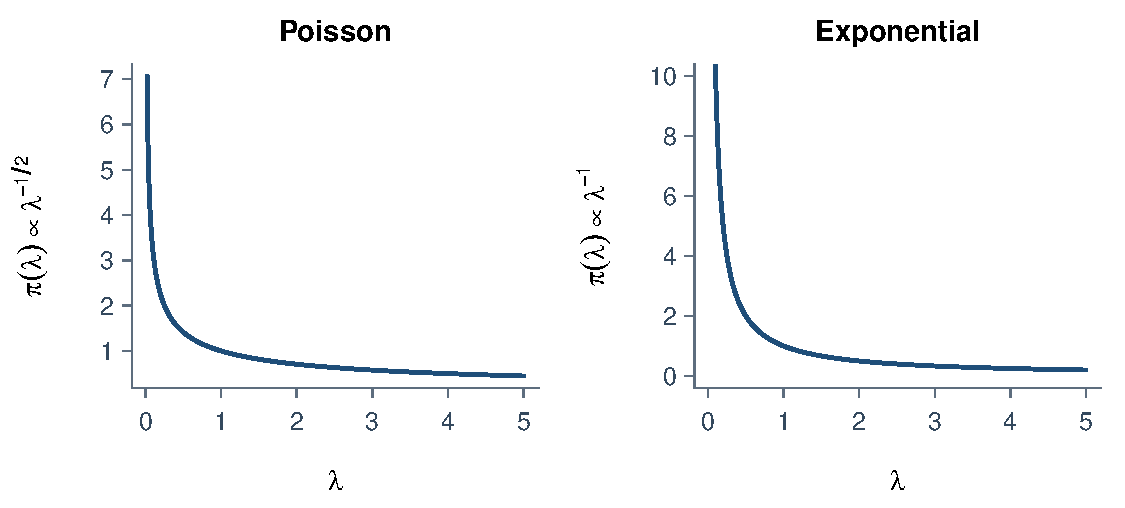
\includegraphics[width=0.85\linewidth]{ex19_20_jeffreys.pdf}\end{center}
\step{(b) Proper?} $\int_0^\infty\lambda^{-1/2}\dd\lambda=\big[2\sqrt\lambda\big]_0^\infty=\infty$. \textbf{Improper} (the problem is the upper tail).
\step{(c) Posterior.}
\[
p(\lambda\mid Y)\propto\lambda^{Y}e^{-\lambda}\lambda^{-1/2}=\lambda^{(Y+1/2)-1}e^{-\lambda}\ \Rightarrow\ \lambda\mid Y\sim\dist{Gamma}\big(Y+\tfrac12,\ 1\big).
\]
A Gamma needs shape $>0$ and rate $>0$; shape $Y+\frac12>0$ for every $Y\in\{0,1,2,\dots\}$.

\begin{answer}
(a) $\pi(\lambda)\propto\lambda^{-1/2}$. \quad (b) Improper. \quad (c) $\lambda\mid Y\sim\dist{Gamma}(Y+\frac12,1)$, proper for \textbf{every} $Y\ge0$, including $Y=0$.
\end{answer}

\begin{takeaway}
The Jeffreys prior is the improper ``$\dist{Gamma}(\frac12,0)$''. It is the default prior used in Exercise 21.
\end{takeaway}

% ================================================================= Exercise 20
\exercise{2.20 --- Jeffreys prior for the exponential rate}

\begin{problem}{20}
Say $Y|\lambda\sim\dist{Gamma}(1,\lambda)$.
\begin{enumerate}[(a)]
\item Derive and plot the Jeffreys prior for $\lambda$.
\item Is this prior proper?
\item Derive the posterior, and give conditions on $Y$ to ensure it is proper.
\end{enumerate}
\end{problem}

\begin{restate}
Same as Exercise 19 but for an exponential waiting time with rate $\lambda$.
\end{restate}

\begin{keyidea}
$\dist{Gamma}(1,\lambda)$ is the exponential with rate $\lambda$: $f(y\mid\lambda)=\lambda e^{-\lambda y}$, $y>0$.
\end{keyidea}

\solution
\step{(a)} $\log f=\log\lambda-\lambda Y$, $\frac{\partial^2}{\partial\lambda^2}\log f=-\frac{1}{\lambda^2}$ (no $Y$ left), so $I(\lambda)=\frac1{\lambda^2}$ and
\[
\pi(\lambda)\propto\frac1\lambda,\qquad\lambda>0
\]
(right panel of the figure in Exercise 19).
\step{(b)} $\int_0^\infty\lambda^{-1}\dd\lambda=\big[\log\lambda\big]_0^\infty$ diverges at \emph{both} ends. \textbf{Improper.}
\step{(c)}
\[
p(\lambda\mid Y)\propto\lambda e^{-\lambda Y}\cdot\lambda^{-1}=e^{-\lambda Y}\ \Rightarrow\ \lambda\mid Y\sim\dist{Gamma}(1,\ Y)=\dist{Exponential}(Y).
\]
This is proper iff the rate $Y>0$. Since $Y$ is a continuous positive variable, $Y>0$ with probability 1. ($Y=0$ would give $p\propto1$, improper.)

\begin{answer}
(a) $\pi(\lambda)\propto1/\lambda$. \quad (b) Improper. \quad (c) $\lambda\mid Y\sim\dist{Gamma}(1,Y)$, proper iff $Y>0$.
\end{answer}

\begin{takeaway}
$1/\lambda$ is the classic scale-invariant prior (flat on $\log\lambda$). It is the Jeffreys prior for any scale or rate parameter.
\end{takeaway}

% ================================================================= Exercise 21
\exercise{2.21 --- A default analysis of one Poisson count}

\begin{problem}{21}
Assume the model $Y|\lambda\sim\dist{Poisson}(\lambda)$, and we observe $Y=10$. Conduct a Bayesian analysis of these data with default prior distribution.
\end{problem}

\begin{restate}
With a single count of 10 and no prior information, use an objective prior and summarise the posterior.
\end{restate}

\begin{keyidea}
The default (objective) choice is the Jeffreys prior $\pi(\lambda)\propto\lambda^{-1/2}$ from Exercise 19, giving $\lambda\mid Y\sim\dist{Gamma}(Y+\frac12,1)$.
\end{keyidea}

\solution
\step{Posterior.} $\lambda\mid Y=10\sim\dist{Gamma}(10.5,\ 1)$.
\step{Summaries.} Mean 10.5, SD $\sqrt{10.5}=3.24$, 95\% interval $(5.14,\ 17.74)$.
\begin{center}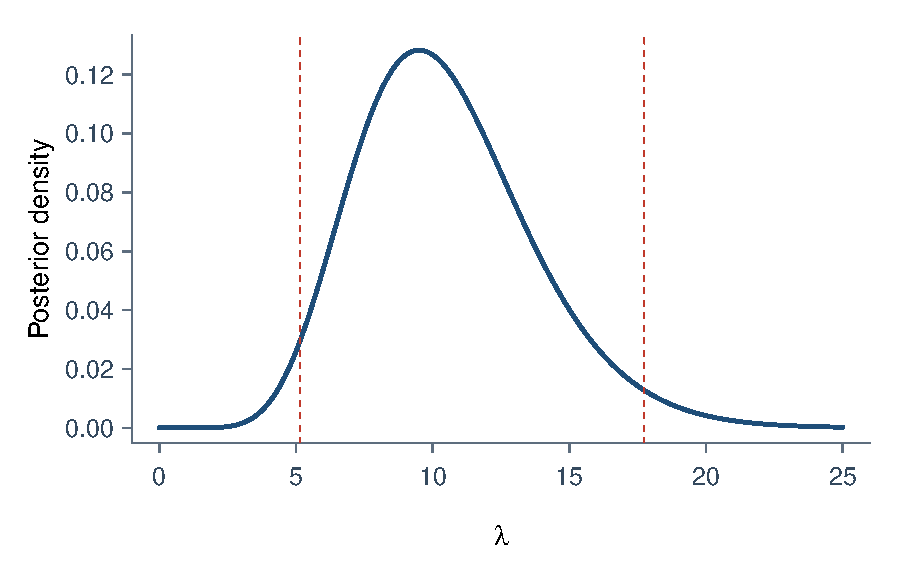
\includegraphics[width=0.66\linewidth]{ex21_posterior.pdf}\end{center}
\step{Comparison with other ``default'' priors.}
\begin{center}
\begin{tabular}{lccc}\toprule
Prior & Posterior & Mean & 95\% interval\\\midrule
Jeffreys $\propto\lambda^{-1/2}$ & $\dist{Gamma}(10.5,1)$ & 10.50 & (5.14, 17.74)\\
Flat $\propto1$ & $\dist{Gamma}(11,1)$ & 11.00 & (5.49, 18.39)\\
$\dist{Gamma}(0.01,0.01)$ & $\dist{Gamma}(10.01,1.01)$ & 9.91 & (4.75, 16.93)\\\bottomrule
\end{tabular}
\end{center}

\begin{answer}
Jeffreys prior $\Rightarrow\lambda\mid Y\sim\dist{Gamma}(10.5,1)$: posterior mean 10.5, SD 3.2, 95\% credible interval $(5.1,\ 17.7)$.
\end{answer}

\begin{takeaway}
With a single observation, ``default'' priors still differ by about half a unit in the mean. Default does not mean irrelevant --- report the choice.
\end{takeaway}

% ================================================================= Exercise 22
\exercise{2.22 --- HOV lane survey: Jeffreys vs.\ empirical Bayes}

\begin{problem}{22}
The data in the table below are the result of a survey of commuters in 10 counties likely to be affected by a proposed addition of a high occupancy vehicle (HOV) lane.
\begin{center}
\small
\begin{tabular}{ccc|ccc}\toprule
County & Approve & Disapprove & County & Approve & Disapprove\\\midrule
1 & 12 & 50 & 6 & 15 & 8\\
2 & 90 & 150 & 7 & 67 & 56\\
3 & 80 & 63 & 8 & 22 & 19\\
4 & 5 & 10 & 9 & 56 & 63\\
5 & 63 & 63 & 10 & 33 & 19\\\bottomrule
\end{tabular}
\end{center}
\begin{enumerate}[(a)]
\item Analyze the data in each county separately using the Jeffreys prior distribution, and report the posterior 95\% credible set for each county.
\item Let $\hat p_i$ be the sample proportion of commuters in county $i$ that approve of the HOV lane (e.g., $\hat p_1=12/(12+50)=0.194$). Select $a$ and $b$ so that the mean and variance of the $\dist{Beta}(a,b)$ distribution match the mean and variance of the sample proportions $\hat p_1,\dots,\hat p_{10}$.
\item Conduct an empirical Bayesian analysis by computing the 95\% posterior credible sets that results from analyzing each county separately using the $\dist{Beta}(a,b)$ prior you computed in (b).
\item How do the results from (a) and (c) differ? What are the advantages and disadvantages of these two analyses?
\end{enumerate}
\end{problem}

\begin{restate}
Estimate approval in each county two ways: on its own with an objective prior, and with a prior estimated from all counties together. Compare.
\end{restate}

\begin{keyidea}
Binomial Jeffreys prior: $\dist{Beta}(\frac12,\frac12)$, giving $\dist{Beta}(Y_i+\frac12,\ n_i-Y_i+\frac12)$. Empirical Bayes: estimate the prior from the data (moment matching, as in Exercise 13), then use it for every county.
\end{keyidea}

\solution
\step{(a) Jeffreys analysis.}
Each county separately: $\theta_i\mid Y_i\sim\dist{Beta}(Y_i+\frac12,\ n_i-Y_i+\frac12)$. The 95\% intervals are in the left half of the table below.

\step{(b) The empirical prior.}
$\bar{\hat p}=0.480$, $\V(\hat p_i)=0.02026$. Then $a+b=\frac{0.48(0.52)}{0.02026}-1=11.32$, so
\[
a=5.43,\qquad b=5.89\qquad(\text{prior mean }0.48,\ \text{worth about 11 respondents}).
\]
\step{(c) Empirical Bayes analysis.}
Each county separately with the $\dist{Beta}(5.43,5.89)$ prior: $\theta_i\mid Y_i\sim\dist{Beta}(5.43+Y_i,\ 5.89+n_i-Y_i)$ (right half of the table).
\begin{center}
\small
\begin{tabular}{cc c cc cc}\toprule
 & & & \multicolumn{2}{c}{(a) Jeffreys} & \multicolumn{2}{c}{(c) Empirical Bayes}\\\cmidrule(lr){4-5}\cmidrule(lr){6-7}
County & $n_i$ & $\hat p_i$ & mean & 95\% interval & mean & 95\% interval\\\midrule
1 & 62 & 0.194 & 0.198 & (0.110, 0.305) & 0.238 & (0.148, 0.341)\\
2 & 240 & 0.375 & 0.376 & (0.316, 0.437) & 0.380 & (0.321, 0.440)\\
3 & 143 & 0.559 & 0.559 & (0.478, 0.639) & 0.554 & (0.475, 0.631)\\
4 & 15 & 0.333 & 0.344 & (0.140, 0.584) & 0.396 & (0.222, 0.586)\\
5 & 126 & 0.500 & 0.500 & (0.414, 0.586) & 0.498 & (0.415, 0.582)\\
6 & 23 & 0.652 & 0.646 & (0.449, 0.820) & 0.595 & (0.429, 0.751)\\
7 & 123 & 0.545 & 0.544 & (0.457, 0.631) & 0.539 & (0.455, 0.623)\\
8 & 41 & 0.537 & 0.536 & (0.386, 0.682) & 0.524 & (0.390, 0.657)\\
9 & 119 & 0.471 & 0.471 & (0.383, 0.560) & 0.471 & (0.387, 0.557)\\
10 & 52 & 0.635 & 0.632 & (0.499, 0.755) & 0.607 & (0.485, 0.723)\\\bottomrule
\end{tabular}
\end{center}
\begin{center}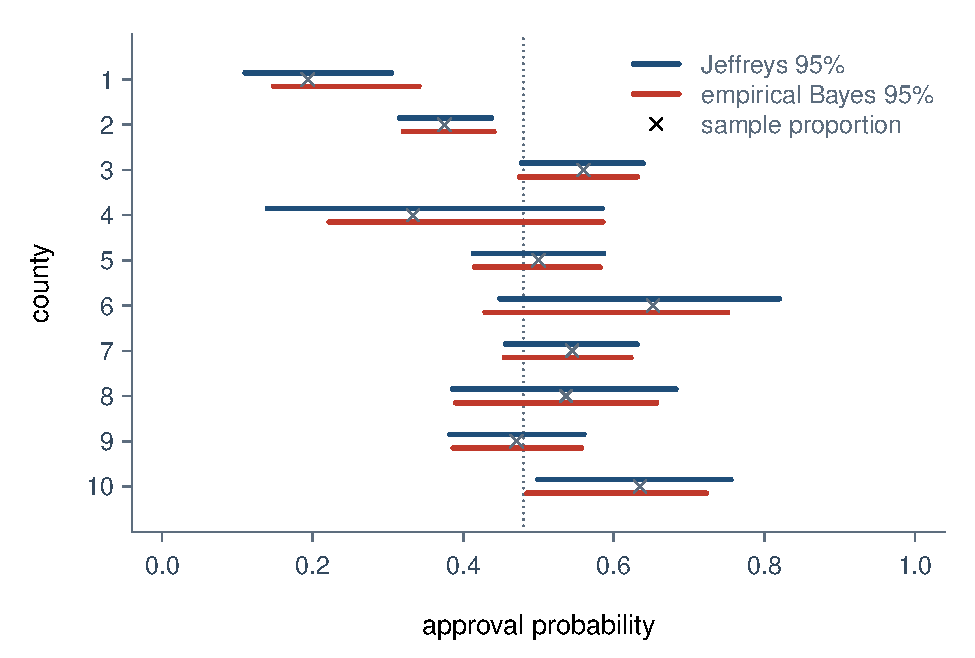
\includegraphics[width=0.75\linewidth]{ex22_intervals.pdf}\end{center}

\step{(d) Comparison.}
\begin{itemize}
\item \textbf{Shrinkage}: empirical Bayes pulls every estimate toward the overall 0.48, most strongly for small counties (county 4: $0.344\to0.396$; county 6: $0.646\to0.595$) and hardly at all for large ones (county 2).
\item \textbf{Precision}: EB intervals are narrower (average width 0.216 vs 0.237).
\item \textbf{Jeffreys} --- advantages: objective, each county stands alone, no assumption that counties are similar. Disadvantages: ignores useful information from other counties; very wide intervals for small counties.
\item \textbf{Empirical Bayes} --- advantages: borrows strength across counties, better estimates on average (especially for small $n_i$). Disadvantages: uses the data twice (to build the prior and to update it) and treats $a,b$ as known, so its intervals are somewhat too narrow; it assumes the counties are exchangeable.
\end{itemize}

\begin{answer}
(a) Jeffreys intervals: see table. \quad (b) $a=5.43$, $b=5.89$. \quad (c) EB intervals: see table.\\
(d) EB shrinks small counties toward 0.48 and narrows intervals (borrowing strength), at the cost of ignoring uncertainty in $(a,b)$. The fully Bayesian fix is a \emph{hierarchical model} with priors on $a$ and $b$ (Section 2.2 / Chapter 7).
\end{answer}

\begin{takeaway}
Empirical Bayes is a practical halfway house between ``each county alone'' and ``all counties identical''. The amount of shrinkage is driven by the data: here the counties differ a lot (variance 0.02), so the prior is weak (11 pseudo-respondents).
\end{takeaway}

\end{document}
